\documentclass[a4paper,12pt,oneside,final]{extbook}

\usepackage[utf8]{inputenc}
\usepackage[T1]{fontenc}

\usepackage{graphicx}
\usepackage{times}
\usepackage[english,swedish]{babel}

\usepackage{geometry}

\geometry{
 margin=20mm
}

\usepackage{fancyhdr}

\usepackage{titling}
\title{Bruse - en webbdatabas för filhantering\\Projektrapport, TNM094}
\author{Grupp J\\Erik Olsson\\Ronja Grosz\\Klas Eskilson\\Daniel Rönnkvist\\Therése Komstadius}

\frenchspacing
\setlength{\parindent}{0pt}
\parskip 5pt

\setcounter{secnumdepth}{3}

\usepackage{color}
\definecolor{rltred}{rgb}{.5,0,0}
\definecolor{rltgreen}{rgb}{0,.5,0}
\definecolor{rltblue}{rgb}{0,0,1}

\usepackage[pdftex,
 colorlinks=true,
 urlcolor=rltblue,       % \href{...}{...} external (URL)
 filecolor=rltgreen,     % \href{...} local file
 linkcolor=rltred,       % \ref{...} and \pageref{...}
 citecolor=rltgreen,     % \cite{...}
 pdftitle={},
 pdfauthor={},
 pdfsubject={Projektrapport, TNM094},
 pdfkeywords={},
 pdfpagemode=,
 pdfstartview=FitH,
 bookmarks=true,
 bookmarksopen=false,
 bookmarksnumbered=true
        ]{hyperref}


\begin{document}

\pagestyle{empty}
\thispagestyle{empty}

\frontmatter

\maketitle

\pagestyle{fancy}

\chapter{Sammanfattning}
Den här rapporten beskriver hur en webbdatabas för filhantering utvecklades i kursen Medietekninskt Kandidatprojekt, TNM094, vid Linköpings universitet. Syftet med projektet var att gruppen skulle följa ett agilt arbetssätt för att uppnå kundens krav. Kundens främsta krav var att databasen skulle användas för att lagra och strukturera personlig information som dokument, bilder och musik. Dessa filer skulle sedan taggas med ett eller flera nyckelord för att kunna söka reda på informationen snabbare. Serversystemet utvecklades i ramverket Ruby on rails och databasens klientsida utvecklades i ramverket Angularjs.

\tableofcontents

\cleardoublepage
% \phantomsection
\addcontentsline{toc}{chapter}{\listfigurename}
\listoffigures

\cleardoublepage
% \phantomsection
\addcontentsline{toc}{chapter}{\listtablename}
\listoftables

\chapter{Typografiska konventioner}
Följande typografiska konventioner används i denna rapport.

\begin{table}[h]
  \begin{centering}
    \begin{tabular}{|l|l|l|}
    \hline
    \textbf{Utseende} & \textbf{Förklaring} & \textbf{Exempel} \\
    \hline
    % krusiv
    \emph{Kursiv text} & Engelska termer & Systemets \emph{models} används för... \\
    \hline
    % monospace
    \texttt{Fast teckenbredd} & Klasser och tekniska komponenter & Systemets \emph{model} \texttt{Identity} används för... \\
    \hline
    \end{tabular}
    \caption[Table caption text]{Typografiska konventioner i rapporten}
    \label{table:type}
  \end{centering}
\end{table}

\begin{table}[h]
  \begin{centering}
    \begin{tabular}{|l|l|l|}
    \hline
    \textbf{Förkortning} & \textbf{Förklaring} \\
    \hline
    API & Application Program Interface \\
    \hline
    CSS & Cascading Style Sheets \\
    \hline
    HTML & HyperText Markup Language \\
    \hline
    SDK & Software Development Kit \\
    \hline
    \end{tabular}
    \caption[Table caption text]{Ofta användna förkortningar}
    \label{table:abbr}
  \end{centering}
\end{table}

\mainmatter


\chapter{Inledning}
\label{ch:inledning}
Eftersom mycket information idag finns i elektronisk form är det viktigt att kunna lagra denna information på ett bra sätt. Ofta används flera olika lagringstjänster och användaren har dålig översyn på var alla filer ligger och vad de heter. Därför är det önskvärt att skapa ett system där en användare kan få åtkomst till olika typer av filer, från olika lagringstjänster på ett snabbt och smidigt sätt.

\section{Bakgrund}
Idén till detta projekt fick kunden av boken \textit{Getting things done} \cite{gettingthingsdone}. I boken presenteras principer för att organisera filer på ett annorlunda sätt jämfört med den vanliga mappstrukturen. Kunden hade som önskemål att enkelt kunna sortera filer och skapa en egen hierarki med hjälp av att ge varje fil en eller flera taggar. Med taggar åsyftades ett eller flera ord som för användaren hade en koppling till filen. På detta sätt kunde användaren komma åt filerna med hjälp av en begränsande sökning istället för att behöva leta sig igenom en djup mappstruktur för att hitta önskat objekt.

\section{Syfte}
Syftet med projektet är att gruppen ska utveckla en webbtjänst för lagring av filer som användaren snabbt ska kunna komma åt via ett sökfält. Sökningen begränsas genom att söka efter taggar eller metadata som den eftersökta filen innehåller. Tjänsten ska vara användarvänlig så att vem som helst ska kunna ha nytta av den. Det ska både gå att lagra sina lokala filer och synkronisera med andra lagringstjänster. Poängen med att synkronisera andra lagringstjänster till en webbtjänst är att användaren kan hantera alla sina uppladdade filer på ett och samma ställe.

För att utveckla den önskade slutprodukten jobbade gruppen enligt utvecklingsmetodiken Scrum. Syftet med att använda Scrum var att tillämpa ett agilt arbetsmönster. Agil utveckling innebär att utvecklarna arbetar efter att ständigt ha en fungerande produkt, så att kontinuerlig återkoppling med kund kan ske. Detta för att säkerställa kundens nöjdhet och för att utveckla ett flexibelt system som förblir relevant. \cite{softwareeng}

Denna rapport redogör för utvecklandet av detta projekt, dess framgångar och dess nederlag. Rapporten tar upp detaljer kring den tekniska implementationen, vad som genomförts och vad som skulle genomförts om mer tid funnits.

\section{Frågeställning}
Arbetet med systemet och denna rapport har kretsat kring ett par centrala frågeställningar.

\textbf{Hur ska en webbdatabas struktureras för att sökning efter sparade objekt ska kunna levereras enligt en användares förväntningar gällande hastighet och resultat för webbtjänster med liknande funktionalitet?}

För ett databasfilsystem är sökning en central komponent. Användaren ska enkelt och utan att behöva vänta, hitta det denne letar efter. Då en databas växer utgör antalet rader i den ett potentiellt problem för sökningar - många rader kod skall gås igenom utav servern. Frågan handlar alltså om hur systemet kan utvecklas för att redan tidigt tackla detta. Hur går det att säkerställa att användarens sökord snabbt genererar resultat, oavsett hur komplex sökfrågan är? Och hur kan användarens söktext användas för att hitta filer utifrån exempelvis taggar och filtyper?

\textbf{Hur går det att säkerställa att en användares information som lagras i en webbdatabas inte är tillgänglig för någon som inte är den specifika användaren eller har blivit  auktoriserad av den specifika användaren?}

Säkerhet är ett ständigt känsligt ämne då webbtjänster diskuteras. Ämnet är dessutom extra känsligt då ett system ämnar att lagra en användares personliga och potentiellt känsliga uppgifter. Hur går det att säkerställa att ingen obehörig person får tillgång till användarens filer? Och hur kan systemet ge ett tryggt intryck?

\textbf{Hur kan filer i en webbdatabas presenteras i en webbapplikation på ett sätt som gör de överskådliga, hanterbara och lättillgängliga för en användare, i en filstruktur utan kataloger eller annan hierarki?}

Denna fråga handlar om hur databasbaserade filsystem på webben kan presenteras. Systemet ska gärna klara av användare som har flera hundra sparade filer, både ur prestanda- och användarvänlighetsperspektiv. Hur mycket information kan presenteras utan att det blir överväldigande?

\textbf{På vilket sätt kan en webbtjänsts användargränssnitt utformas för att demonstrera all funktionalitet ett system besitter och göra det intuitivt för en användare?}

Systemet ska göra som användaren förväntar sig, trots att filstrukturen kan vara något användaren är ovan vid. Hur går det att anpassa en webbtjänst till hur exempelvis filhanteringsprogrammet användaren är van vid beter sig?

\section{Avgränsningar}
Utgående från kundens krav riktar sig installation av systemet mot en användare som har tillräckligt stor teknisk kompetens för att kunna hantera ett UNIX baserat operativsystem. Vidare utvecklas systemet också för en slutanvändare med viss erfarenhet av liknande system. Det är alltså inte anpassat för ovana datoranvändare.

\chapter{Relaterat arbete}
I projektet har metoder och ramverk för såväl arbete som mjukvara använts. Nedan kommer en förklaring på de största delarna som använts och implementerats.

\section{Scrum}
Scrum är ett ramverk som innefattar olika roller, aktiviteter och tekniker för att förenkla utvecklingsprocessen. Det finns nyckelroller inom teamet för att se till att alla delar ses över utan att lägga allt ansvar på en individ. Det finns även en rad förutbestämda möten och uppdateringar som är till för att ge hela gruppen bra överblick och en chans att påverka arbetet.

Inom Scrum delas hela utvecklingsperioden upp i tidsrutor, så kallade sprintar. Dessa är förutbestämda tidsperioder som strukturmässigt är uppbyggda på samma sätt varje omgång. De inleds med ett planeringsmöte där fokus och mål för förestående sprint bestäms. Inför varje ny arbetsdag hålls ett kort scrummöte där alla i teamet får presentera det de gjort sen senast och vad de ska göra kommande arbetsdag. Detta för att alla ska få en bra bild över hur arbetet ligger till tidsmässigt och om det finns några problem som måste lösas.

I slutet av varje sprint hålls två möten. En sprintgranskning och en sprintåterblick. Sprintgranskningen går ut på att alla i utvecklingsteamet sätter sig ned, eventuellt även med kund, och går igenom vad som åstadkommits under senaste sprint. Arbetet demonstreras och utvecklarna svarar på eventuella frågor, presenterar problem och hur dessa har lösts. Detta möte är till för att utvärdera de tekniska lösningar som applicerats. Sprintåterblicken är ett internt möte för utvecklingsteamet. Även här ska senaste arbetet utvärderas men ur ett socialt perspektiv istället för ett tekniskt. Här ska gruppens relationer diskuteras, hur användandet av valda verktyg fungerat och det finns även tillfälle för alla enskilda individer att utvärdera egen arbetsinsats.

Alla krav som finns för projektet sparas i en så kallad backlogg. Det är en rörlig lista där krav rangordnas utefter prioritet. När ett krav blir mer aktuellt eller mer väldefinierat flyttas det uppåt i listan. \cite{scrumguide}

\section{Mjukvaruramverk}
Två stora mjukvaruramverk som använts i projektet är Ruby on Rails samt Angularjs.

\subsection{Ruby och Ruby on Rails}
Ruby on Rails är ett ramverk skrivet i språket Ruby \cite{rubylang}. Ramverket är skrivet med öppen källkod som används utav flera stora tjänster på nätet, bland annat mikrobloggstjänsten Twitter, sammarbetsverktyget Github och boendeförmedlingstjänsten Airbnb. Ramverket är skrivet enligt designmönstret MVC. Detta står för \textit{model}, \textit{view}, \textit{controller} och är ett sätt att strukturera ett projekts logik på sådant vis att olika komponenter har egna tydliga platser och syften.

I Ruby on Rails skapar utvecklaren \textit{models}. Detta är en samling klasser vars syfte är att hantera data som användaren eller systemet interagerar med, och fungerar som ett lager ovanpå databasen. Ett exempel på en \textit{model} kan vara en klass för användare eller filer. Samtliga databasoperationer sker genom systemets \textit{models}. En \textit{model} skrivs i Ruby med syntaxen \textit{CamelCase} medans klasstabellerna i databasen är namngivna med \textit{snail}\_\textit{case}.

Den komponent som sköter interaktionen mellan det som användaren interagerar med och systemets \textit{models} är systemets \textit{controllers}. Här finns logik för att hantera användares handlingar och hämta data från systemets \textit{models}. Ett exempel kan vara att användaren klickar på en knapp i webbläsaren. Syftet med knappen är att visa en viss data. Användarens handling skickas till en \textit{controller} som tar emot vad det är för data som användaren efterfrågar och hämtar den datan från en \textit{model}. Här finns också logik för att hantera undantag, till exempel om datan saknas. Den \textit{controller} som anropats skickar sedan resultatet av användarens begäran vidare till användaren.

Det som användaren i sin tur interagerar med är systemets \textit{views}. Här presenteras det som systemets \textit{controllers} producerat. Knappen som användaren trycker på, i exemplet i stycket ovan, skapas i en \textit{view}. Här kan det också finnas länkar, texter, textfält och alla andra komponenter som utgör det som renderas av en webbläsare.

En mer överskådlig figur för hur data och interaktioner generellt sett färdas genom ett MVC-system visas i figuren nedan. Data transporteras från \textit{models} till \textit{views} via \textit{controllers}. Interaktioner färdas mellan \textit{views} och \textit{models} via \textit{controllers} och direkt mellan \textit{controllers} och \textit{views} samt mellan \textit{controllers} och \textit{models}, se figur \ref{fig:mvc1}.

\begin{Figure}
  % center it!
  \centering
    % adjust width as you like, include image from optional folder
    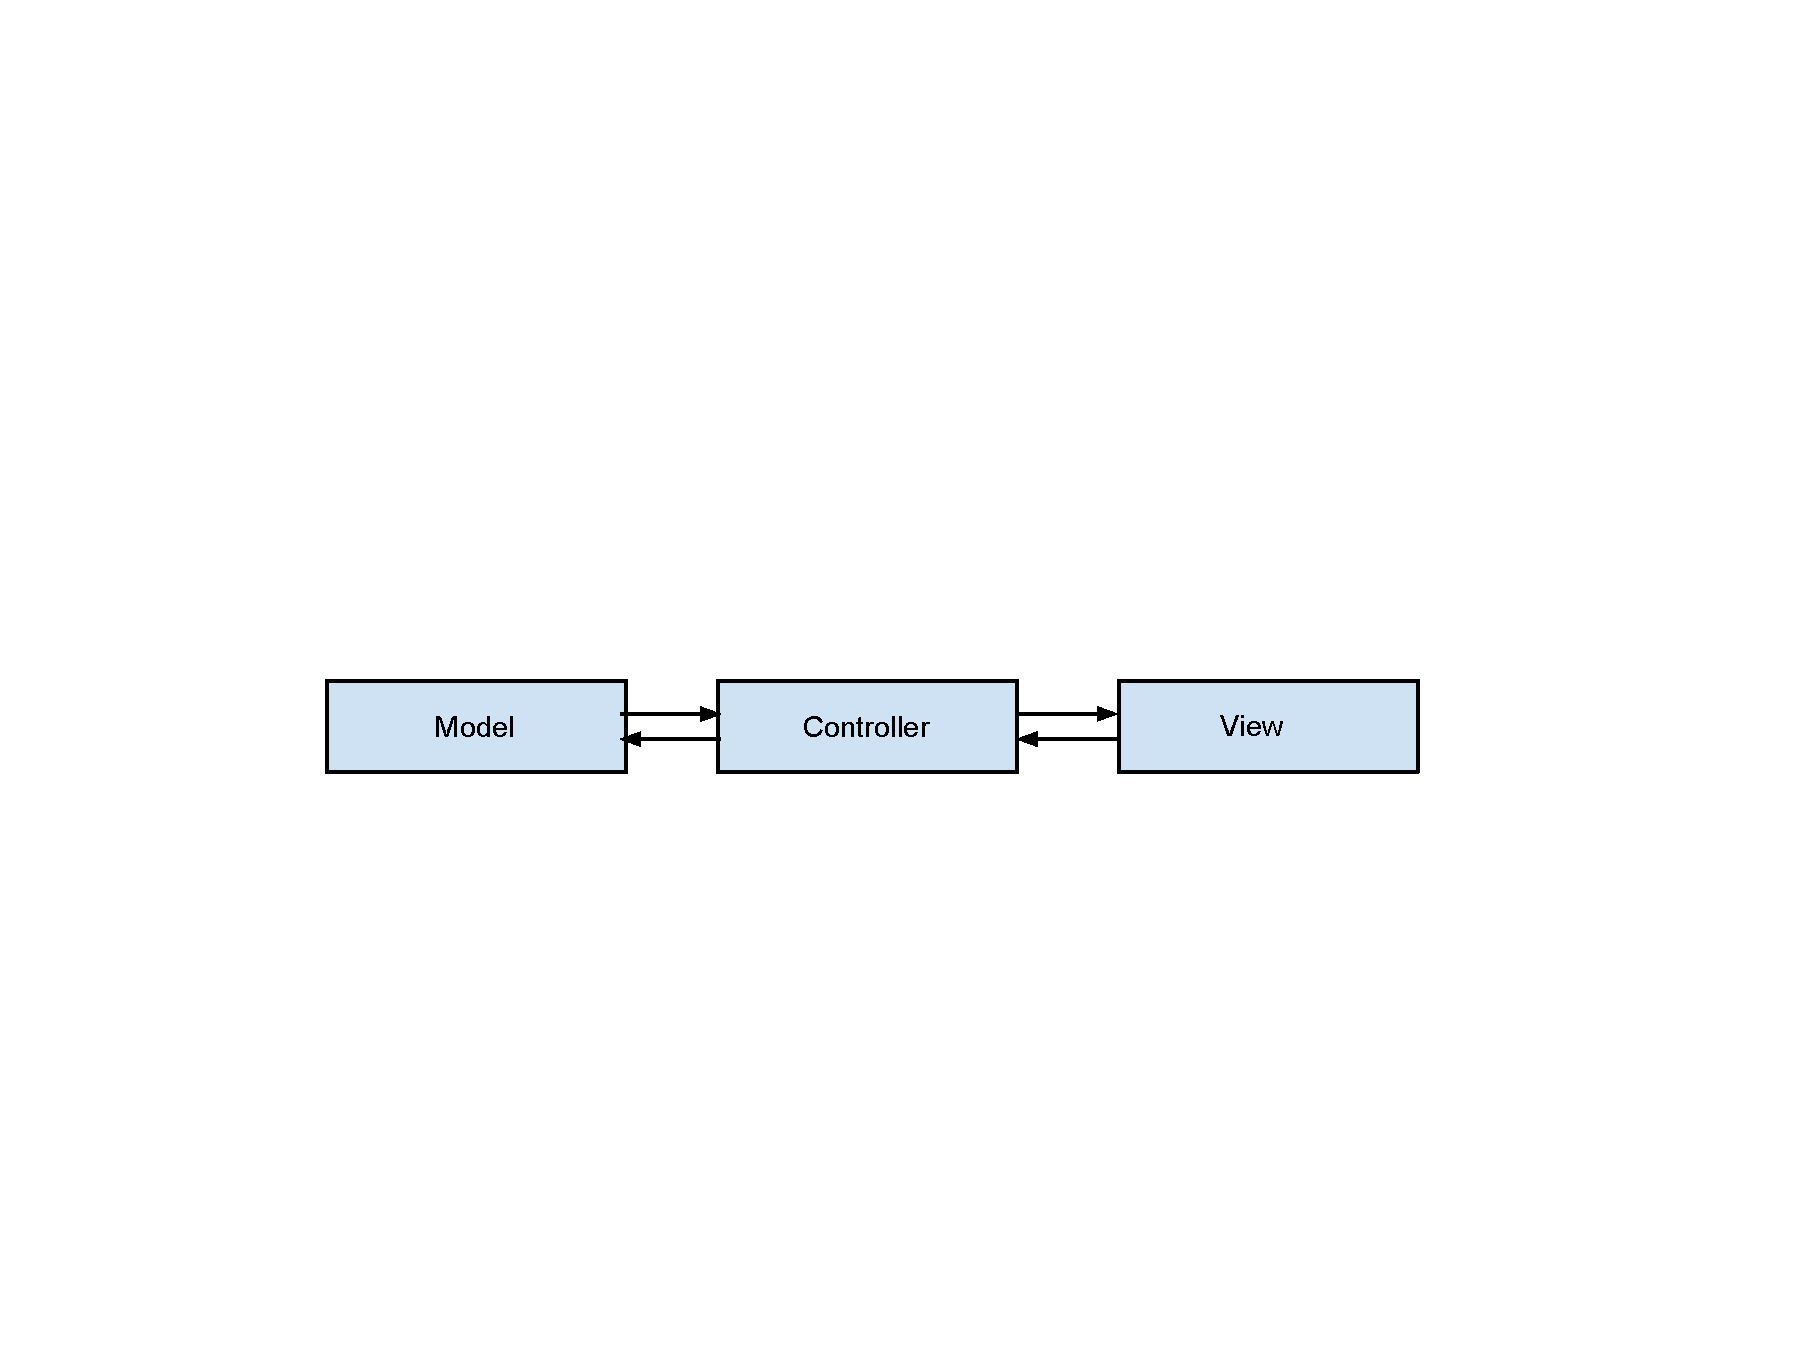
\includegraphics[width=0.8\textwidth]{figures/mvc1.pdf}
    % caption! change the label ref to what you want
    \captionof{figure}{\emph{MVC-systemets struktur.}\label{fig:mvc1}}
\end{Figure}

En annan figur som snarare fokuserar på MVC ur ett användarperspektiv visas i figur \ref{fig:mvc2}.

\begin{Figure}
  % center it!
  \centering
    % adjust width as you like, include image from optional folder
    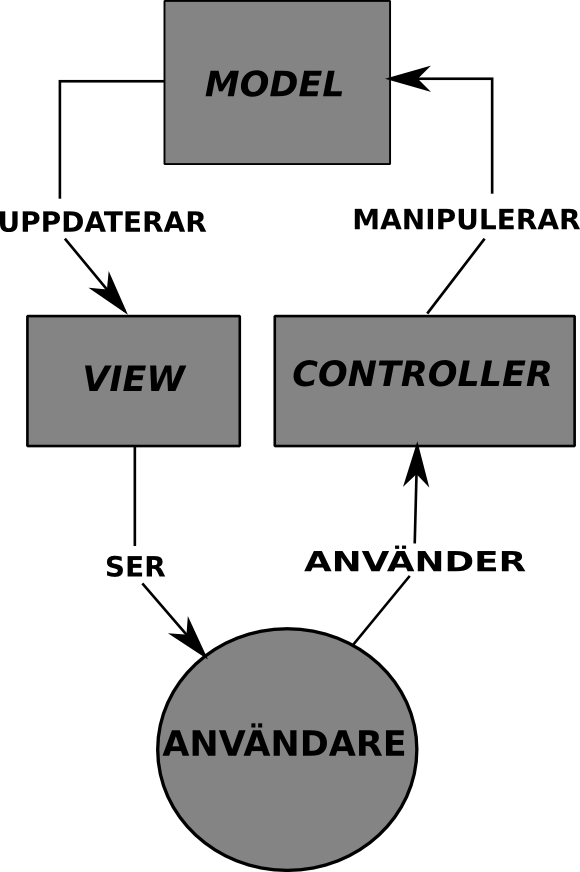
\includegraphics[width=0.5\textwidth]{figures/mvc2.png}
    % caption! change the label ref to what you want
    \captionof{figure}{\emph{MVC ur ett användarperspektiv.}\label{fig:mvc2}}
\end{Figure}

\subsection{Angularjs}
Angularjs är ett så kallat MVW-ramverk, vilket står för \textit{Model}-\textit{View}-\textit{Whatever} \cite{angularjs}. För att effektivt använda detta ramverk bör även systemet byggas upp efter den designen. Då \textit{whatever} innebär att det finns flera olika typer av sätt att kontrollera eller manipulera data på, kan varje komponent i systemet få specialanpassade lösningar.

I Angularjs finns så kallade \textit{factories}. Detta är en samling hjälpfunktioner vars syfte är att undvika kodupprepning och göra det enkelt för koden att återanvändas på flera platser i systemet.

\section{Övrig tredjepartsmjukvara}
Då Ruby on Rails och Angularjs är mjukvara med öppen källkod har det bildats globala nätverk kring dessa ramverk. Många tillägg, verktyg och bibliotek har skrivits för att underlätta utvecklandet i dessa ramverk.

För att underlätta för utvecklare har Ruby on rails byggts med en mängd olika verktyg. Möjligheten finns även för utvecklare att bygga egna verktyg som kallas för \textit{gems} och är ofta fria att använda och även de skrivna med öppen källkod.

För att fortsätta bidra till detta nätverk kring Ruby on Rails och Angularjs utvecklades även projektet med öppen källkod, för att kunna dela de lösningar som tagits fram.

\section{Taggar och sökning} \label{sec:tags}
För att uppnå en effektiv sökstruktur i en databas finns det två olika metoder. Den första metoden kallas professionell indexering och är hierarkisk. Den andra metoden kallas folksonomi vilket bygger på att taggar sätts på innehållet utan någon särskild hierarki. Sammanfattat kan de beskrivas som “\emph{Indexering strävar efter precision medan taggning strävar efter hantering}” \cite{tagging}.

Genom professionell indexering ramas den eftersökta informationen in med hjälp av huvudkategorier och underkategorier. Det går alltid att ta sig fram i databasens olika kataloger och till slut hitta den sökta filen. Folksonomi går ut på att hitta den eftersökta filen genom taggar. Nyckelorden behöver inte följa någon speciell hierarki eller struktur sinsemellan.

\section{Gränssnitt}
För att designa ett användavänligt gränssnitt kan Normans Principer\cite{norman} tillämpas för att åstadkomma en god användarupplevelse. Dessa utgår ifrån sex punkter: synlighet, återkoppling, begränsningar, mappning, konsekvens och affordans.

\subsection{Synlighet}
Det är viktigt att utforma en design som gör att användaren känner sig trygg i gränssnittet. Användaren ska helst kunna förutspå vad som händer när denne klickar på en ikon eller en rubrik. Ikoner ska tala för sig själv, till exempel en ikon med en soptunna betyder kasta och en penna betyder redigera. För att göra det lättare för användaren att hitta det mest relevanta på sidan kan tomma utrymmen användas \cite{whitespace}. Dessa tomma utrymmen är grafiska utrymmen som inte innehåller någon typ av information. De är till för att skapa mer “luft” i gränssnittet. Detta gör att användares fokus begränsas kring ett visst område och det blir lättare att navigera.

\subsection{Återkoppling}
Att ständigt ge återkoppling till vad som sker eller vad som har skett gör att användare känner sig tryggare i systemet. Dialogrutor, laddningssymboler och felmeddelande är exempel på viktig återkoppling \cite{whitespace}. Utan en laddningssymbol kan användaren få känslan av att ingenting händer och går därför kanske tillbaka och upprepar steget, vilket förstör hela processen.

\subsection{Begränsningar}
För att användaren inte ska göra oönskade saker i systemet eller ha för många alternativ, är det en bra idé att begränsa alternativen \cite{whitespace}. Till exempel förvirrar för många menyalternativ på en hemsida.

\subsection{Mappning}
Mappning innebär att liknande innehåll samlas på samma plats för att hålla en god struktur \cite{whitespace}. Användare ska snabbt kunna hitta filens tillhörande funktioner. Detta kan åstadkommas genom att visa alternativen i anslutning till filerna.

\subsection{Konsekvens}
För att göra det lättare för användaren att minnas hur denne använde en funktion är det bra att ha en liknade design på hela hemsidan. Det blir lätt rörigt för användren om designen inte följer ett mönster. Att använda sig av samma teckensnitt och färgschema hjälper till att hålla sidan konsekvent \cite{whitespace}.

\subsection{Affordans}
Affordans betyder att ett objekt själv ska kunna beskriva vad det ska användas till. Till exempel är det tydligt att det går att hänga kläder på en klädkrok och ingen ytterligare beskrivning krävs \cite{whitespace}. Samma sak gäller på en hemsida. Användaren ska inte behöva fundera över vad som kommer hända när denne klickar på exempelvis en papperskorg, det vill säga något kommer att raderas.

\section{Databaserat filsystem}
Ett databasbaserat filsystem använder sökning för att hitta filer genom metadata eller nyckelord. De flesta filsystem använder kataloglagring. Ett examensarbete på University of Twente i Nederländerna hade som uppgift att undersöka om ett databasbaserat filsystem kan ersätta filsystem med kataloglagring med avseende på användbarhet och förmåga att lära sig att använda systemet \cite{twente}. Genom användartester drogs slutsatsen att ett databasbaserat filsystem presterade bättre utifrån dessa aspekter.

\chapter{Webbdatabas för hantering av filer}
I detta kapitel kommer de olika delar som utvecklingen av systemet bestod av att presenteras.

\section{Inledande möten}
Projektet inleddes med ett antal interna gruppmöten där projektets vision diskuterades utifrån projektets beskrivning. Diskussionen ledde till många frågor, dels kring tekniska bitar och dels kring kundens krav. På första kundmötet besvarades dessa frågor i den mån kunden kunde. Kunden hade inte alltid en bestämd åsikt om hur ett problem skulle lösas och lät därför utvecklarna hitta en lösning. Efter kundmötet hölls ett nytt gruppmöte där projektvisionen förtydligades och tekniska lösningar diskuterades och ritades upp.

I inledningen av projektet diskuterades det mycket om hur systemet skulle utvecklas. Faktorer som språk och ramverk togs upp. Beslutet som fattades var att språket Ruby och ramverket Ruby on Rails skulle användas som grundstomme i projektet. Vidare användes också Javascript och ramverket Angularjs för att göra upplevelsen av systemet snabbare för användaren.

När gruppen hade en tydlig idé om hur databasen skulle se ut och vilken teknik som skulle användas skrevs en projektplan (se bilaga []) som skulle ligga till grund för arbetsrutinerna, ansvarsfördelningen och tidsplanneringen (se bilaga []).

\section{Hantering och strukturering av databaser}
Systemet använder sig utav en SQL-databas, där SQL står för \textit{Structured Query Language}. Det är ett programmeringsspråk för att lagra, bearbeta och hämta information i en databas \cite{sqlenc}.

\subsection{Databasstruktur}
Inledningvis togs en grundläggande databastruktur fram. Databasen innehöll användare, användares olika externa konton (till exempel Dropbox eller Google Drive), filer och taggar, se figur \ref{fig:relations}.

\begin{Figure}
  % center it!
  \centering
    % adjust width as you like, include image from optional folder
    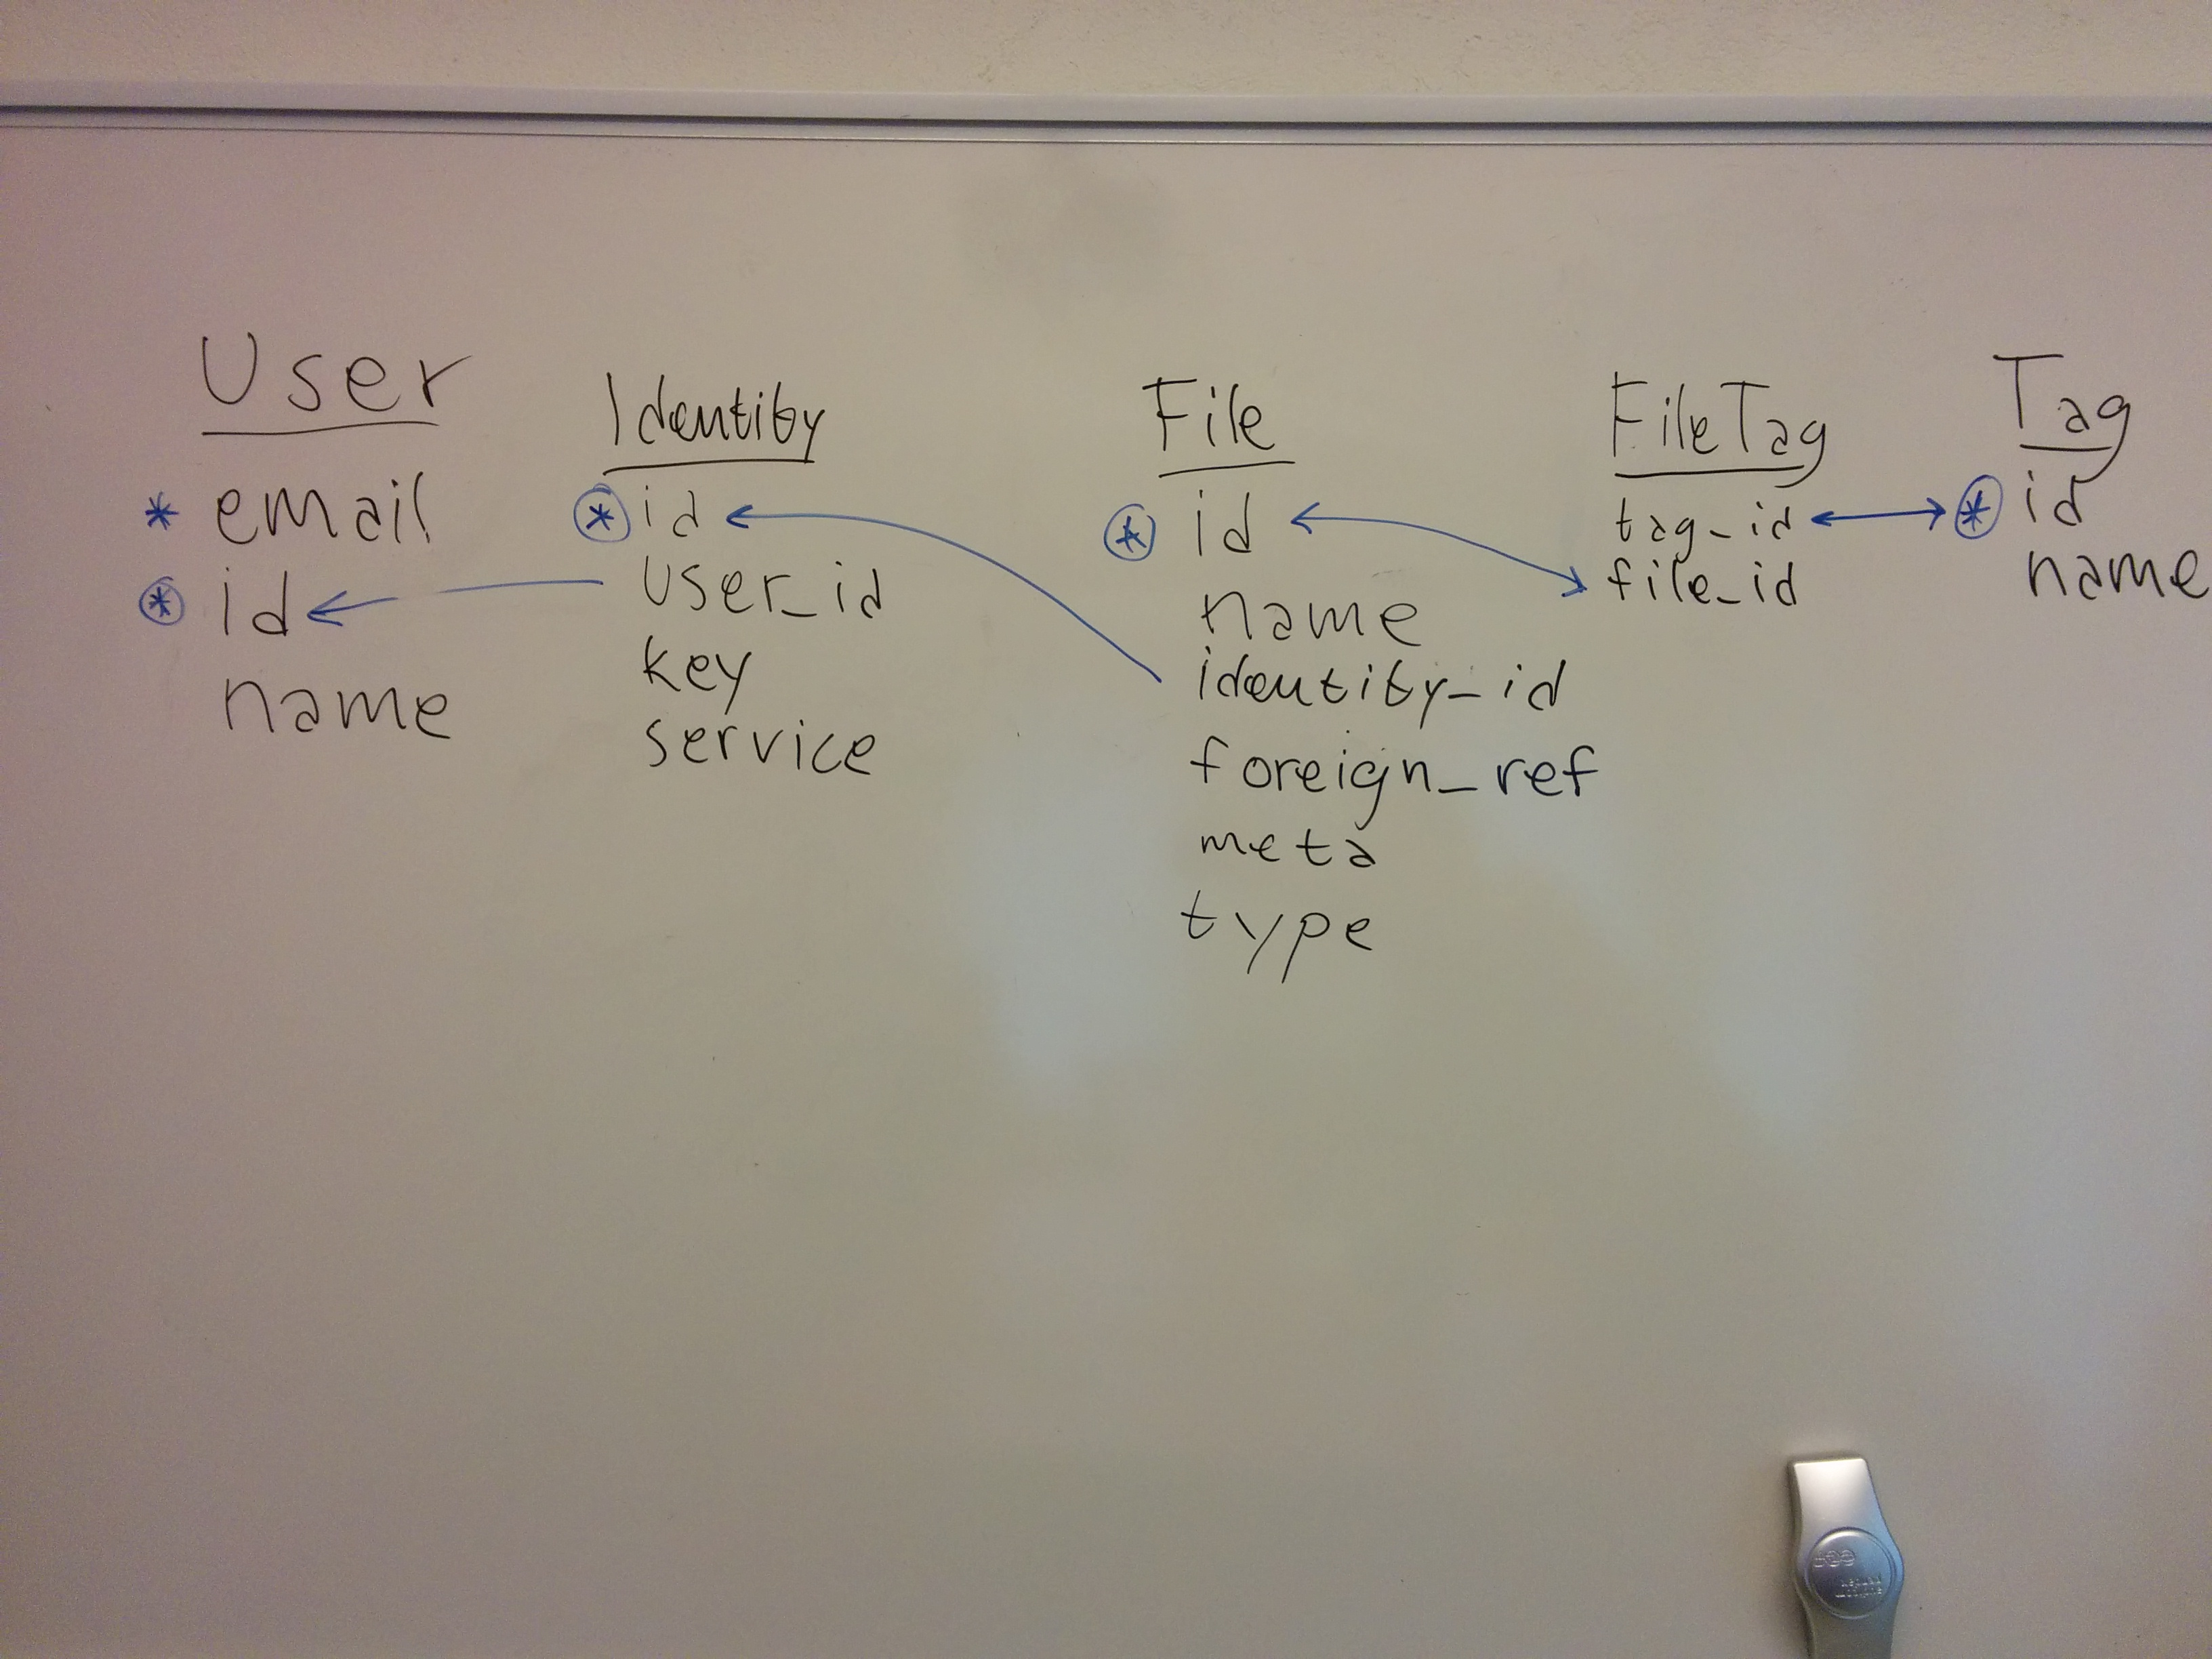
\includegraphics[width=0.8\linewidth]{figures/relations.jpg}
    % caption! change the label ref to what you want
    \captionof{figure}{\emph{Inledande databasstruktur.}\label{fig:relations}}
\end{Figure}

\subsection{Databashantering}
En stor komponent utav Ruby on Rails är modulen som heter \texttt{ActiveRecord}. Detta är en modul vars syfte är att förenkla databashantering \cite{objrel} och skapades efter ett designmönster med samma namn \cite{proar}. Istället för att skriva databasfrågor manuellt kan en utvecklare använda systemets \texttt{ActiveRecord}-\textit{models} för att förenkla arbetet. Rent praktiskt kan detta innebära att ersätta SQL-frågan “\texttt{SELECT * FROM table WHERE column1=’value’}” med “\texttt{Table.where(column1: ‘value’)}”.

Med hjälp av detta kunde komplexa relationer mellan olika tabeller i databasen förenklas, och en objektorienterad struktur med Ruby-klasser skapades utifrån tabellerna. En extern nyckel i en SQL-tabell kan i sin \texttt{ActiveRecord}-form liknas med en pekare till ett annat objekt. Detta ledde till att arbetet kunde skyndas på, och att avancerad kunskap om SQL-frågor inte var nödvändig för utvecklingen av sidan.

I och med att Rails \texttt{ActiveRecord}-modul hade inbyggt stöd för SQL-databaser användes dessa för systemets relationella tabeller. Mer specifikt användes SQL-databasen Postgresql i systemet. En fördel med Postgresql är dess indexering som bygger på bland annat B-trees \cite{indexes}. (Redogörelse för indexeringsmetoder och datastrukturerna bakom dem går bortom räckvidden för denna rapport.) Denna indexeringsmetod möjliggjorde snabba sökningar baserat på olika parametrar (exempelvis namn eller etiketter), vilket ansågs viktigt för systemet.

\section{Systemarkitektur}
Systemet kan sägas vara uppdelat i två huvudsakliga delar. Dels finns det som körs på en server i Ruby-kod och dels finns det som körs hos klienten (webbläsaren) i Javascript.

\subsection{Javascript och Angularjs}
För att skapa ett responsivt system, i bemärkelsen att det var snabbt för användaren, valdes det att implementera mycket utav funktionaliteten hos klienten med hjälp av Javascript. Systemet innehåller många olika komponenter som ska interagera med varandra. Ett exempel är då flera filer ska listas med verktyg för att hantera filen, samtidigt som den filen har flera taggar som också ska kunna hanteras.

För att skriva Javascriptkod användes Coffeescript, vilket är ett språk som kompileras till Javascript. Coffeescript bidrar till en mer kompakt kod, har en syntax som är mer lik Rubys syntax och ämnar att underlätta vissa bitar av Javascript. \cite{coffee}

Ramverket Angularjs användes för hanteringen av datan i gränssnittet. \textit{Controllers}, \textit{factories}\cite{angularwebb}, och en särskild fil för presentationen av filerna skapades. Funktioner implementerades på klientsidan för att få ett gränssnitt som uppdaterades snabbt när olika operationer utfördes. Operationer som sökning, sortering och visning av filer sköts med hjälp av Angularjs.

Systemets \textit{factories} underlättade också för utvecklingen av vissa av systemets asynkrona komponenter. Asynkront innebär att koden inte nödvändigtvis väntar på att samtliga kodrader exekveras uppifrån och ned. Istället kan vissa funktioner ta den tid de behöver. Resultatet blev ett snabbt system, samtidigt som utvecklaren fick en utmaning att hantera detta på ett bra sätt.

\section{Tredjepartsmjukvara}
Några \textit{gems} som använts under utvecklandet av detta system är:

Byebug, ett avlusningsverktyg som möjliggör för utvecklare att sätta brytpunkter i koden. När systemet kör och stöter på den rad där denna brytpunkt finns pausas systemet. I konsolen kunde sedan variabler granskas och utvecklarna kunde steg för steg följa vilken väg koden följde.

Letter opener, ett verktyg för att hantera e-post som skickas av systemet. Istället för att utvecklaren sätter upp en e-postserver som skickar e-postmeddelandena via den, öppnar Letter opener e-posten i webbläsaren. Detta gjorde att utvecklingen av systemets e-postrelaterade komponenter blev betydligt enklare.

För utvecklandet av Angularjs och annan Javascript användes Chrome Developer Tools och tillägget Angularjs Batarang. Dessa är verktyg som gör det lättare för utvecklare att följa med i vad som händer då de använder webbläsaren Google Chrome. Med funktioner som brytpunkter och möjligheten att bevaka variabler blir utvecklandet betydligt enklare.

\section{Filhantering}
För att hantera tjänstens filer implementerades tre olika fillagringssätt. En modulär filhantering skapades för att lätt kunna implementera fler sätt att lagra filer. Dropbox implementerades först eftersom det ansågs vara ett enkelt sätt att hantera användarens filer. När det väl implementerats upptäcktes det att Dropbox krävde en krypterad anslutning till systemet, vilket kostar pengar. På grund av detta infördes även Google Drive som lagringssätt. Efter ett möte med kunden flyttades fokus till att också implementera lokal fillagring.

\subsection{Dropbox}
Dropbox implementerades med hjälp av Dropbox SDK. SDK står för \textit{Software Development Kit} vilket är en uppsättning av utvecklingsverktyg för mjukvaruutveckling mot specifika ramverk eller programpaket, i det här fallet till utveckling mot Dropbox tjänster. Dropbox SDK ger verktyg för att utveckla nya tjänster som använder sig av Dropbox olika funktioner. Webbtjänsten som utvecklades använder sig av ned- och uppladdning av filer till och från Dropbox. För att nå användarens filer måste en autentisering till Dropbox ske, vilket görs med hjälp av Omniauth, en \textit{gem}.

Med hjälp av Dropbox SDK hämtas metadata för filerna i rot-mappen för att sedan visas för användaren. Om en mapp sedan klickas på hämtas metadatan för filerna i den mappen med hjälp av sökvägen. En fil laddas också ned med hjälp av dess sökväg. För att ladda upp filer till Dropbox krävs det att de läggs till i en existerande mapp eller i rot-mappen. För att hålla filerna som laddats upp till Dropbox samlade, skapas automatiskt en mapp med namnet “Bruse” där filerna lagras.

\subsection{Google drive}
Likt Dropbox användes Google Drive SDK för att kunna använda deras funktionalitet i systemet. För att nå användarens filer krävs en autentisering för att ansluta till användarens konto hos Google Drive. Det här görs med hjälp av två \textit{gems}, Drive SDK samt Omniauth. Filhanteringen sker likt metoden för Dropbox, förutom att Drive inte strukturerar sina filer med hjälp av sökvägar. Varje fil har istället en parameter för \textit{parent} och varje mapp har en parameter \textit{child}, där eventuella filer i mappen lagras. Om en fil ligger i en mapp är mappen filens \textit{parent} och filen är mappens \textit{child}, se figur \ref{fig:parentchild}. För att identifiera det här förhållandet kommer alla filer som ligger i samma mapp ha mappens id i dess parent parameter. Liknande kommer mappens parameter child innehålla alla id tillhörande filer som ligger i mappen.

\begin{Figure}
  % center it!
  \centering
    % adjust width as you like, include image from optional folder
    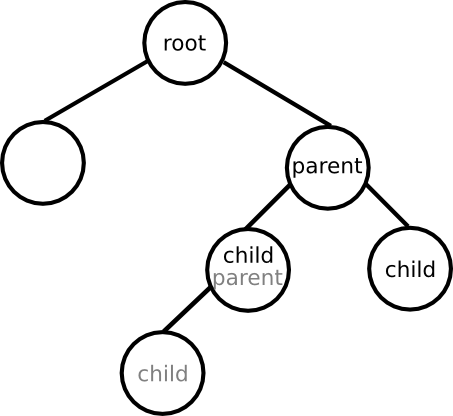
\includegraphics[width=0.5\linewidth]{figures/pcarent2.png}
    % caption! change the label ref to what you want
    \captionof{figure}{\emph{Visar strukturen för parametrarna \textit{parent} och \textit{child} i Google drive.}\label{fig:parentchild}}
\end{Figure}

\subsection{Lokal fillagring} \label{sec:local}
Den lokala filhanteringen infördes för att ge användaren ett alternativ utan extern kostnad och utan filutrymmesbegränsningar från externa tjänster. För att sköta uppladdningen, som är en central del av den lokala filhanteringen i och med att det inte går att importera filer likt från Google Drive eller Dropbox, implementerades en så kallad drag och släpp-uppladdning samt en formulärsuppladdning. Drag och släpp-uppladdningen innebär att användaren kan markera en eller flera filer på sin dator, dra dem till webbläsarfönstret där systemet är öppet och släppa dem. Systemet tar där vid och laddar upp filerna. När servern har tagit emot all uppladdningsdata från webbläsaren får filen ett slumpat filnamn och placeras i en mapp på servern.

\section{Gränssnitt}
För att utveckla gränssnittet användes främst HTML, CSS och Javascript. För att skriva CSS användes verktyget SASS\footnote{http://sass-lang.com/} (\textit{Syntactically Awesome Style Sheets}), vars syfte är att förenkla avancerade stilstrukturer genom att bland annat tillåta loopar, nästlade stilregler samt funktioner i CSS. Javascript användes för att göra gränssnittet snabbare för användaren genom att placera viss logik för utseendet i användarens webbläsare. Detta ledde till att webbläsarens DOM (\textit{Document Object Model}) kunde modifieras, och på så sätt snabbt ändra innehållet som presenteras. För detta användes Angularjs.

Sidans CSS kompletterades av ett par SASS- och CSS-ramverk för att underlätta utvecklandet. Bourbon\footnote{http://bourbon.io} användes för att tillhandahålla smidiga hjälpfunktioner, så kallade \textit{mixins} till SASS. För att kunna fylla tomma rutor i tjänsten användes kolumnsystemet Jeet\footnote{http://jeet.gs}. För att nollställa webbläsares olika standardinställningar, exempelvis länkars färger eller typsnitt, användes Normalize.css\footnote{http://necolas.github.io/normalize.css/}. Ikoner lades till för att göra knappar mer intuitiva vilket biblioteket Font Awesome\footnote{http://fontawesome.io}  användes för. För att visa att systemet laddar hem data, eller skicka data, användes Nprogress \footnote{http://ricostacruz.com/nprogress/}. Vidare användes knappar och textfält från Skeleton  \footnote{http://getskeleton.com}.

CSS-koden strukturerades upp i flera filer för att skapa en mer överskådlig struktur. Strukturen var uppdelad i följande kategorier: knappar, textfält, generell layout-struktur, huvudmeny, länkar, fillistor samt små individuella komponenter.

\section{Testning}\label{sec:4test}
Sedan version 1.9 utav Ruby har standardverktyget för testning varit Minitest \cite{rubychangelog}. Minitest erbjuder många delar som behövs för att kunna hantera testning. Det som användes mest var så kallade \textit{fixtures}, en exempelinstans utav en \textit{model} i systemet. Dessa användes för att säkerställa att systemet producerade de förändringar mot modellen som var väntade. Men även att de \textit{controllers} som fanns i systemet utförde rätt logik beroende på datan.

För att kontinuerligt säkerställa att projektet levde upp till de krav testerna specificerade användes tjänsten Travis CI, som testar att starta systemet och köra dess tester. Varje gång ny kod laddades upp gavs då ett resultat om hur testerna gick. Med denna kontinuerliga uppdatering gick det att via Github följa projektets status utan att ladda ned och starta det.

För testning av gränssnittet krävs dock ett program som kan simulera en webbläsares funktion genom att rendera Javascript, HTML och CSS. Då Travis CI redan hade ett sådant program som heter Phantomjs installerat valdes den. För att integrera Phantomjs med Minitest användes Capybara. Capybara är ett testningsverktyg och finns som tillägg till Minitest. Capybara erbjuder inte bara stöd för rendering utav javascript med Phantomjs utan ger också hjälpfunktioner för att göra tester som simulerar användarbeteende i gränsnittet, något som täcker in stora delar av både servern och gränsnittet.

De tester som utvecklarna lade mest tid på att implementera var tester för \textit{models}, \textit{controllers} samt integrationstester. Integrationstester är tester som testar ett användarbeteende och har väldigt enkla instruktioner, till exempel gå till startsidan och fyll inloggningsformuläret med dessa uppgifter och tryck sedan på logga in. Med dessa tester gavs en helhetsblick och en väldigt stor del av systemet testades med ett och samma test.

Tester skrevs efter att en funktion hade implementerats för att säkerställa att den önskade funktionaliteten skulle hålla i framtida utveckling av andra funktioner.

\section{Utvecklingsmetodik}
Genom att använda Scrum som utvecklingsmetodik gavs en bra grund och tydliga riktlinjer att följa under projektets gång.

\subsection{Roller}
Utvecklingsteamet bestod av fem personer där varje person fick en nyckelroll:

\subsubsection{Scrummästare}
Dennes ansvar innefattade att se till att teamet höll sig till de riktlinjer som fanns, sköta kommunikationen runt de mer administrativa bitarna (boka sal, bestämma arbetsdagar och så vidare) och hålla i scrummöten.

\subsubsection{Produktägare}
Produktägarens ansvar var att hålla kontakten med kund och se till att kundens krav omvandlades till scenarion och uppgifter. Det var även dennes ansvar att hålla ordning i produktbackloggen.

\subsubsection{Kodansvarig}
Dennes ansvar gick ut på att hitta ett bra system för att integrera nya delar i det befintliga systemet och sedan se till att detta system upprätthölls.

\subsubsection{Testansvarig}
Dennes uppgift var att se till att systemet testades för att säkerställa att de krav som fanns uppnåddes och för att kontinuerligt jobba för att upptäcka brister i systemet.

\subsubsection{Dokumentansvarig}
Dokumentansvarig hade till uppgift att säkerställa att projektet blev ordentligt dokumenterat. Det var önskvärt att ha protokoll från kundmöten, gruppmöten med beslutsfattande karaktär och dokumentera skisser och liknande vid diskussioner kring systemets uppbyggnad.

\subsection{Händelser}
Hela utvecklingsperioden delades upp i mindre sprintar. Dessa sprintar hade en förutbestämd tid som inte kunde förlängas även om teamet upplevde att tiden inte räckte till. Varje sprint hade samma struktur. Vid uppstart hölls en sprintplanering där alla i teamet satte sig tillsammans för att gå igenom vilka scenarion från produktbackloggen som skulle ligga till grund i förestående tidsperiod. Det var viktigt att försöka hålla en god balans mellan tid och antalet valda scenarion. Teamet fick tillsammans utvärdera om de ansåg det möjligt att utföra alla scenarion innan sprintens avslut. När samtliga scenarier var valda bröts de ned i mindre delar och formades till specifika uppgifter. Det var önskvärt att hålla dessa uppgifter små och konkreta för att ha möjlighet att genomföra dessa under en arbetsdag.

Inför varje arbetsdag i en sprint höll teamet ett dagligt scrummöte. Detta var ett kort möte på max 15 minuter där alla i teamet stod upp, utan datorer. Varje gruppmedlem fick under detta möte berätta vad de gjorde senast och vad de skulle göra under dagen. Detta gav alla en bra inblick i arbetet och en kort avstämning på hur teamet låg till tidsmässigt.

Den sista arbetsdagen i varje sprint ägnades åt de två avslutande sprintmötena. Det första av dessa var en sprintgranskning. Detta var ett tillfälle då hela teamet kunde diskutera det senaste projektinkrementet och hur arbetet hade fortskridit. Det första som gjordes på dessa möten var att gå igenom de scenarion som fanns inför sprinten och om dessa blivit avslutade. Eftersom målet med varje sprint var att ha en fungerande produkt med de krav som scenarierna representerade, gav denna genomgång en tydlig bild om hur effektivt gruppen arbetat. Nästa del i mötet var att diskutera de problem som uppstått under sprintens gång och hur dessa blivit lösta. Den sista delen av dessa möten ägnades åt att diskutera den dåvarande backloggen, vad som skulle göras härnäst och vilka faktorer som spelade roll inför nästa produktinkrement.

Den sista aktiviteten i varje sprint var en sprintåterblick. Detta var ett möte där gruppen lade fokus på sina egna prestationer, de sociala relationerna i gruppen och de verktyg som använts. Detta var ett tillfälle där alla fick möjlighet att diskutera och påverka dessa aspekter för att jobba mot ett bättre arbetsklimat.

För att kunna skapa en realistisk bild över projektets storlek, vilka tidsramar projektet skulle delas upp i och hur mycket som skulle kunna åstadkommas under projektets gång skapades en tidsplan. För att ge en tydlig bild skapades ett Gantt-schema \cite{softwareeng} som ett kalkylark i teamets gemensamma Google Drive. Där samlades alla dagar i projektperioden. I schemat kunde deadlines, tänkta kundmöten, sprintarna och lediga perioder åskådliggöras på ett smidigt sätt. (BILAGA [])

För att få en överblick över vilken sprint som påbörjats och vilka uppgifter som skulle slutföras användes webbtänsten Trello, se figur \ref{fig:trello}, som scrumboard\cite{scrumboard}. Produktägaren skötte uppdateringen av pruduktbackloggen och sprintbackloggen i denna tjänst. Samtliga i gruppen hade fria händer att påbörja vilken uppgift som helst från sprintbackloggen. För att veta vem som påbörjat en uppgift märktes uppgiften med gruppmedlemmens namn. Övrig dokumentation som till exempel protokoll från sprintåterblick och sprintgranskning sköttes med hjälp av Google Drive. Även skisser på klassdiagram och programfunktionalitet sparades som bilder i Google Drive.

\begin{figure}[!H]
\centering
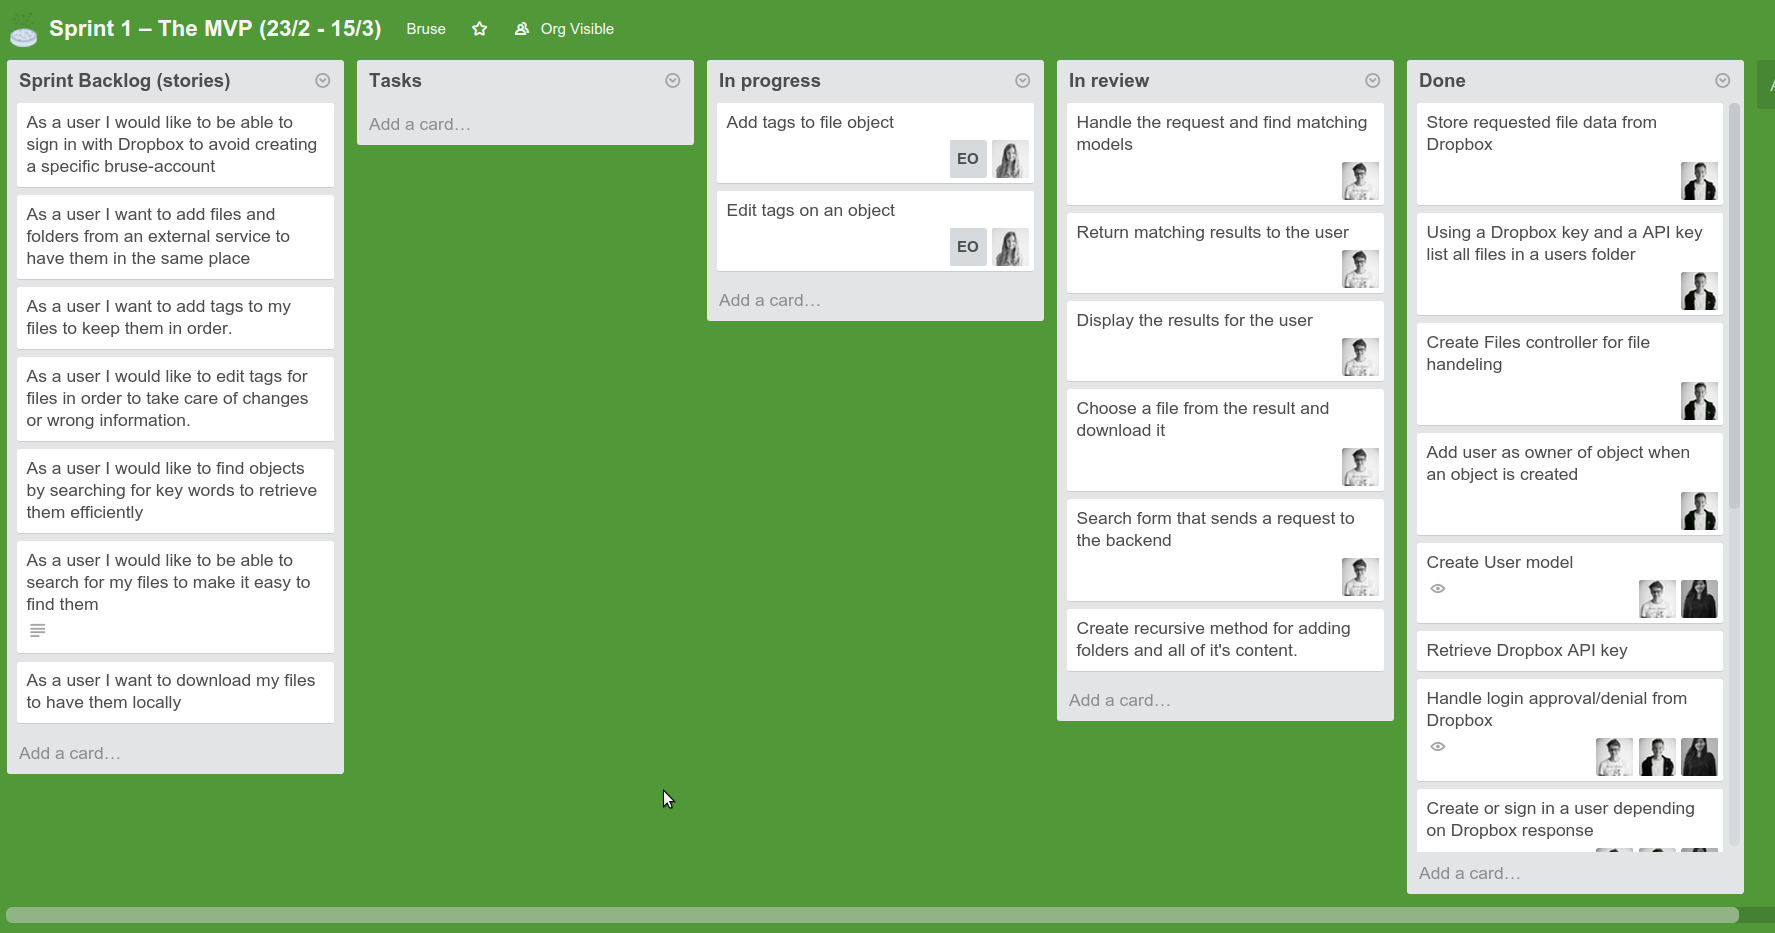
\includegraphics[width=0.8\textwidth]{figures/trello.png}
\caption{Scrumboard över sprint ett.}
\label{fig:trello}
\end{figure}

Här presenteras kort det fokus som fanns för varje sprint. Fullständiga sprintbackloggar går att se i (Bilaga []).

\subsubsection{Sprint 1 - MVP}
Målet med denna sprint var att ha en \textit{Minimum Viable Product}, MVP\cite{mvp} efter sprintavslutet. Något som var funktionellt och kunde visa på de problem som systemet skulle kunna lösa i ett senare skede. Fokus låg på att skapa en användare med Dropbox som fildatabas, importera filer från Dropbox till systemet och skapa nyckelord för filerna.

\subsubsection{Sprint 2 - Utveckla den tekniska funktionaliteten}
Fokus här var att göra filerna lättåtkomliga och sökbara. Dock uppkom det ett problem gällande Dropbox som fildatabas. En kostnad för ett SSL-certifikat (\textit{Secure Sockets Layer}), som används för att visa att en anslutning är krypterad, gjorde att teamet fick ändra riktning efter samråd med kund. Utöver sökningen blev det även fokus på att skapa ett mer modulärt system för att kunna lägga till flera typer av tjänster. Det teamet kom överens om var att implementera Google Drive och även skapa en lokal databas för egen server.

\subsubsection{Sprint 3 - Tänka på användaren}
Under sprint tre hamnade fokus mer på systemets användare än den tekniska funktionaliteten. Ett flöde för systemets användande togs fram [BILD?], sökresultatens visning diskuterades [BILD?] samt utvecklades, och funktionalitet för drag och släpp-uppladdning påbörjades.

\subsubsection{Sprint 4 - Färdig produkt}
I den sista sprinten var det önskvärt att skapa ett användargränssnitt, få klart alla öppna scenarion och förbättra redan implementerad kod.

\section{Versionshantering och kodgranskning}
För versionshantering användes Git i kombination med Github genomgående i projektet. Git är ett distribuerat versionshanteringssystem där samtliga utvecklare har en komplett lokal kopia av hela projektet på dess egna datorer \cite{progit}.

För att underlätta vid konflikter och andra problem som uppstår då parallell utveckling av närliggande delar av projektet skedde användes Gits förgreningsfunktion. Förgreningar är en metod för att lösa problem som uppstår vid en linjär utveckling, där allt måste ske i en viss ordning. Flera utvecklare kunde jobba på olika komponenter utifrån en gemensam grund, och Git organiserade sedan hur dessa kunde sammanfogas på enklast möjliga vis \cite{progit}.

Inom förgreningen implementerades också en metod som populärt kallas \textit{feature branches}, som ungefär kan översättas till funktionalitetsgrenar \cite{gitflow}. Då en ny funktionalitet skulle implementeras i systemet skapade den ansvarige utvecklaren en förgrening. När utvecklaren var klar med det aktuella arbetet, skapades en förfrågan på Github (en \textit{pull request}) om att sammanfoga koden för den nya funktionaliteten med den befintliga. Innan koden sammanfogades fick den ansvarige utvecklaren återkoppling från resterande medlemmar i utvecklingsteamet om de blivande förändringarna och tilläggen. På så sätt skapades en trygghet för utvecklargruppen att det fanns en gemensam förståelse och konsensus kring det som skulle bli en del av den befintliga kodbasen.

\section{Refaktorering}
Refaktorering, det vill säga omstrukturering av kod, skedde med jämna mellanrum då till exempel en \textit{controller} blev för stor eller innehöll för många olika funktionaliteter. Den delades då upp för att tydliggöra vad de olika delarna hanterar. Exempelvis delades \textit{controllern} som hanterar användarnas filer upp i sex delar då den innehöll logik för olika delar av filhanteringen.

\chapter{Resultat}

Nedan presenteras det system som utvecklats.

\section{Installation av systemet}
Ett av kraven från kunden var att kunna installera systemet på sin egna server
och låta det köra därifrån. För att underlätta för kunden vid installationen
skapades en installationsfil som laddar ner systemets filer, fixar
inställningar för databasen och även ställer frågor om vilka
tredjepartstjänster som ska användas. Installationsfilen anpassar sedan
systemet utefter de svar som fås av användaren vid installation. Stegen för
installationen kan ses i figur \ref{fig:installation}.

\begin{figure}[!h]
\centering
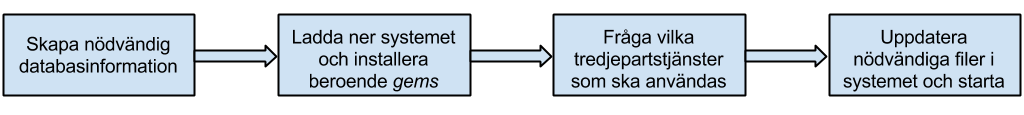
\includegraphics[width=0.8\textwidth]{figures/installation.png}
\caption{De steg som installationsfilen tar för att installera systemet.}
\label{fig:installation}
\end{figure}

\section{Programdesign}

Systemet är uppdelat i två huvudsakliga delar: server och klient.
Javascriptklienten skickar och tar emot data från servern, som presenterar
resultatet i JSON (\emph{Javascript object notation}).

\subsection{Ruby on Rails}\label{sec:ror}

Följande \emph{models} valdes att användas för systemet. Relationerna mellan
dem är specificerade i figur \ref{fig:models}. Modellen \texttt{BruseFile} fick
det namnet eftersom \texttt{File} är ett reserverat ord i Ruby.

\begin{Figure}
  % center it!
  \centering
    % adjust width as you like, include image from optional folder
    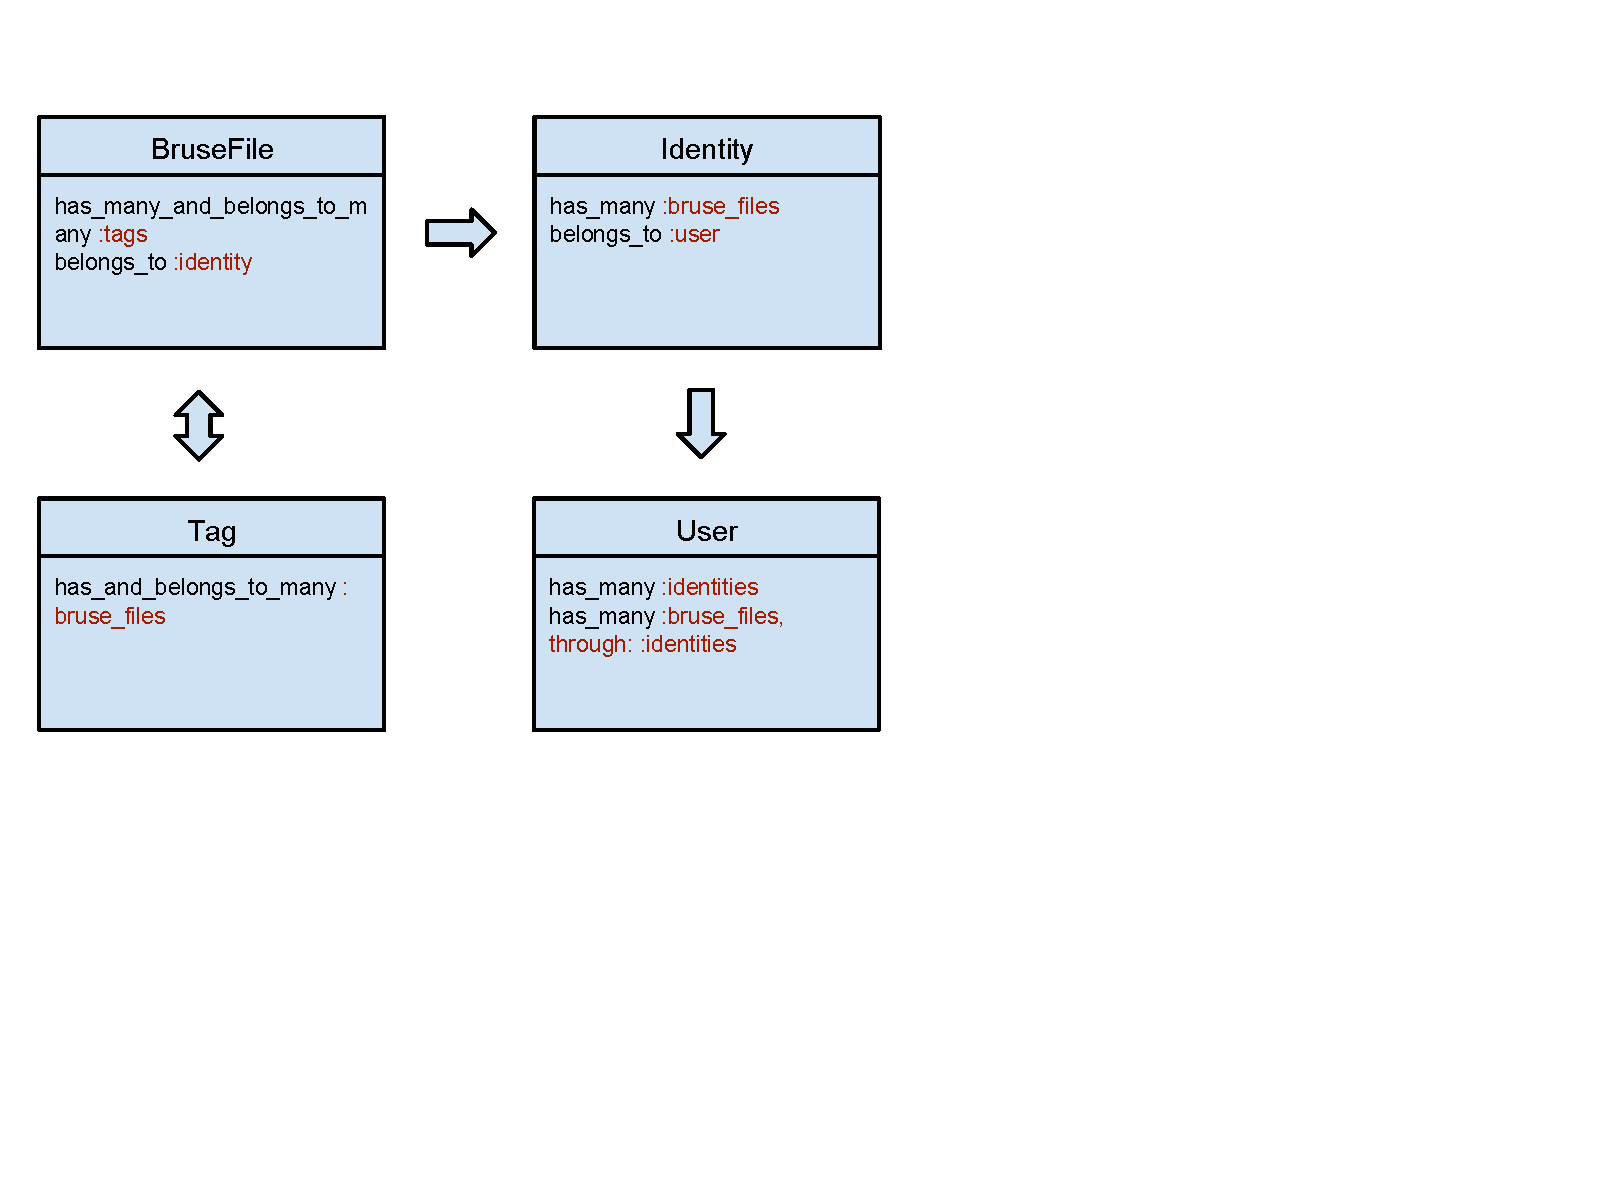
\includegraphics[width=0.7\linewidth]{figures/model.pdf}
    % caption! change the label ref to what you want
    \captionof{figure}{\emph{Systemets \emph{models} och dess relationer.}\label{fig:models}}
\end{Figure}

\texttt{Identity} är en av  systemets viktigaste models. En \texttt{Identity}
är en av tredjepartstjänsterna Google Drive eller Dropbox. Men även den egna
filhanteringen hanteras som en \texttt{Identity} för att hålla det konsekvent
och modulärt. Modellen är viktig för att kunna skilja på vilken
tredjepartstjänst filen tillhör och kunna hantera den därefter.

För att kunna presentera en fil och dess taggar äger \texttt{BruseFile} flera
taggar, men för att även kunna lista filer beroende på en tagg äger varje tagg
flera \texttt{BruseFiles}. Rails löser relationen mellan dessa två genom att
skapa en tabell som heter \texttt{bruse\_files\_tags} enligt figur
\ref{fig:filestags}.

\begin{Figure}
  % center it!
  \centering
    % adjust width as you like, include image from optional folder
    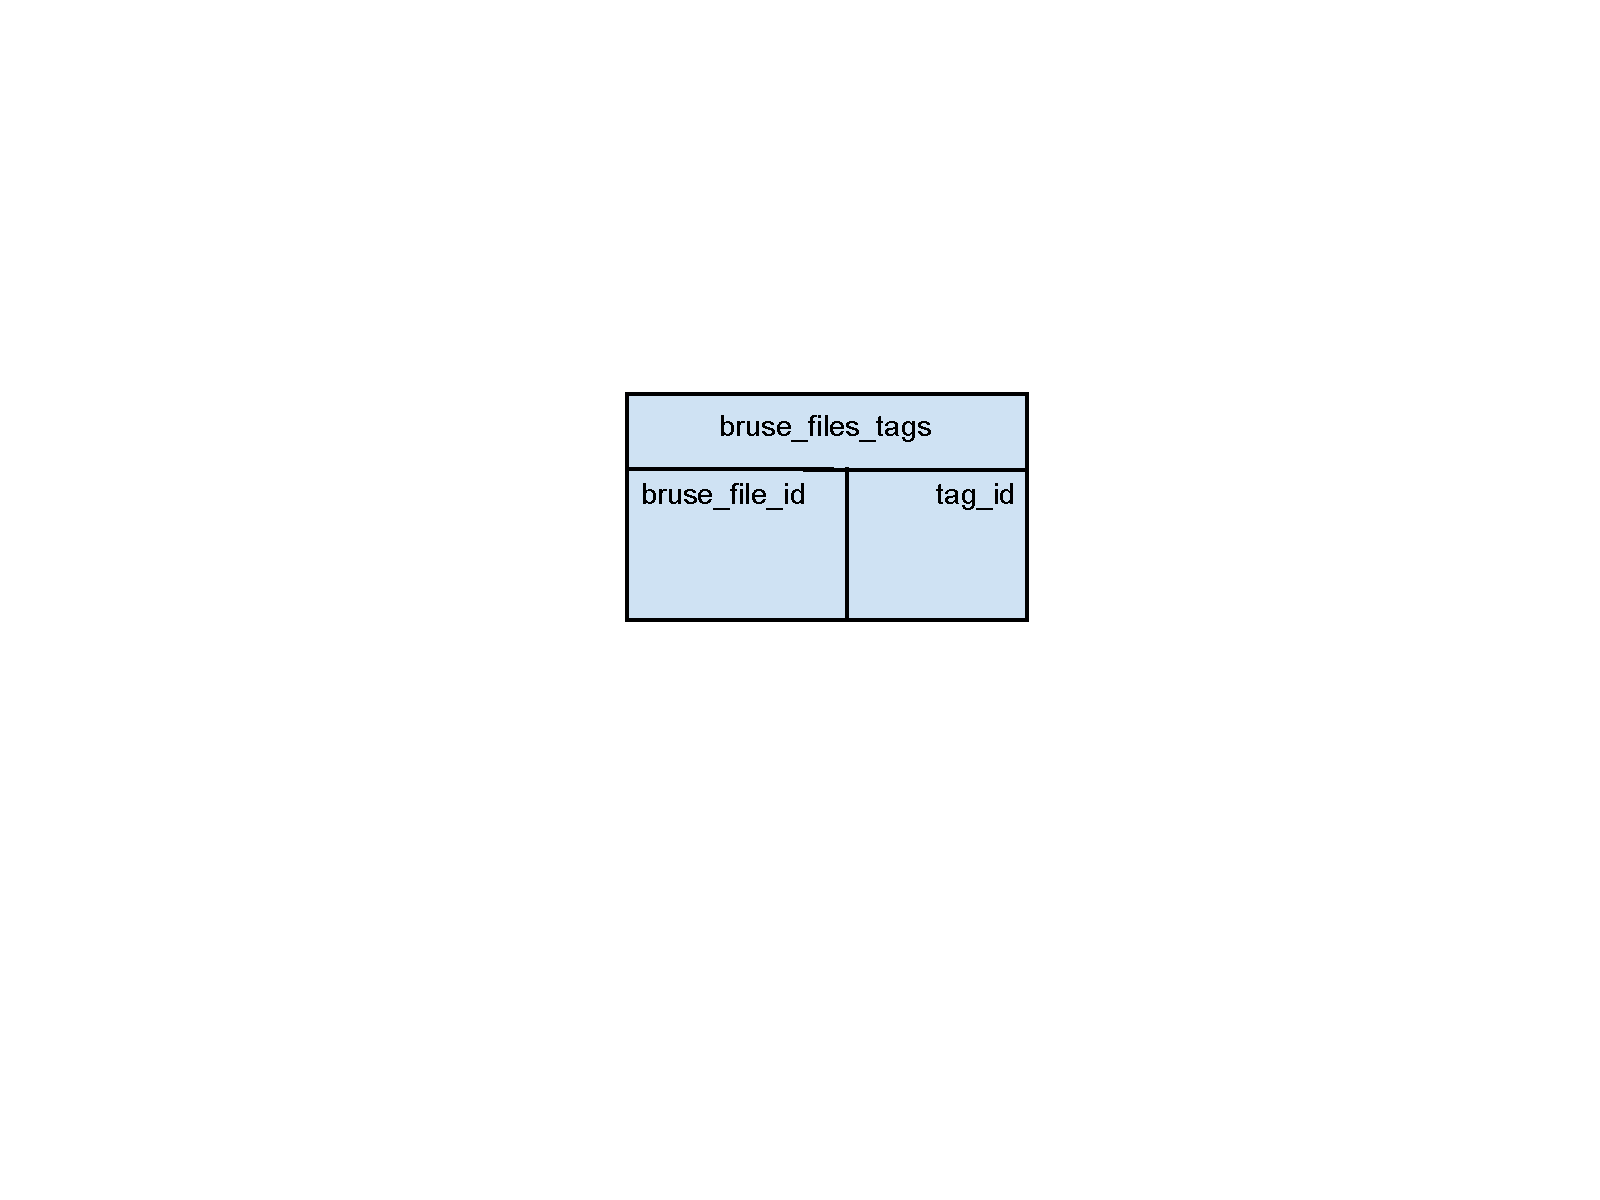
\includegraphics[width=0.3\linewidth]{figures/filestags.pdf}
    % caption! change the label ref to what you want
    \captionof{figure}{\emph{Relation mellan \texttt{BruseFiles} och \texttt{Tags}.}\label{fig:filestags}}
\end{Figure}

Den \emph{controller} som hanterade \texttt{BruseFiles} delades först upp i tre
delar efter en första refaktorering för att sedan bli sex vid utökad
funktionalitet och ytterligare refaktorering. Detta för att filhanteringen
behandlar olika aspekter och behöver då delas upp för att skapa en tydlig
översikt. I figur \ref{fig:filescontroller} beskrivs de olika \emph{controllers}
som används för \texttt{BruseFiles}.

\begin{Figure}
  % center it!
  \centering
    % adjust width as you like, include image from optional folder
    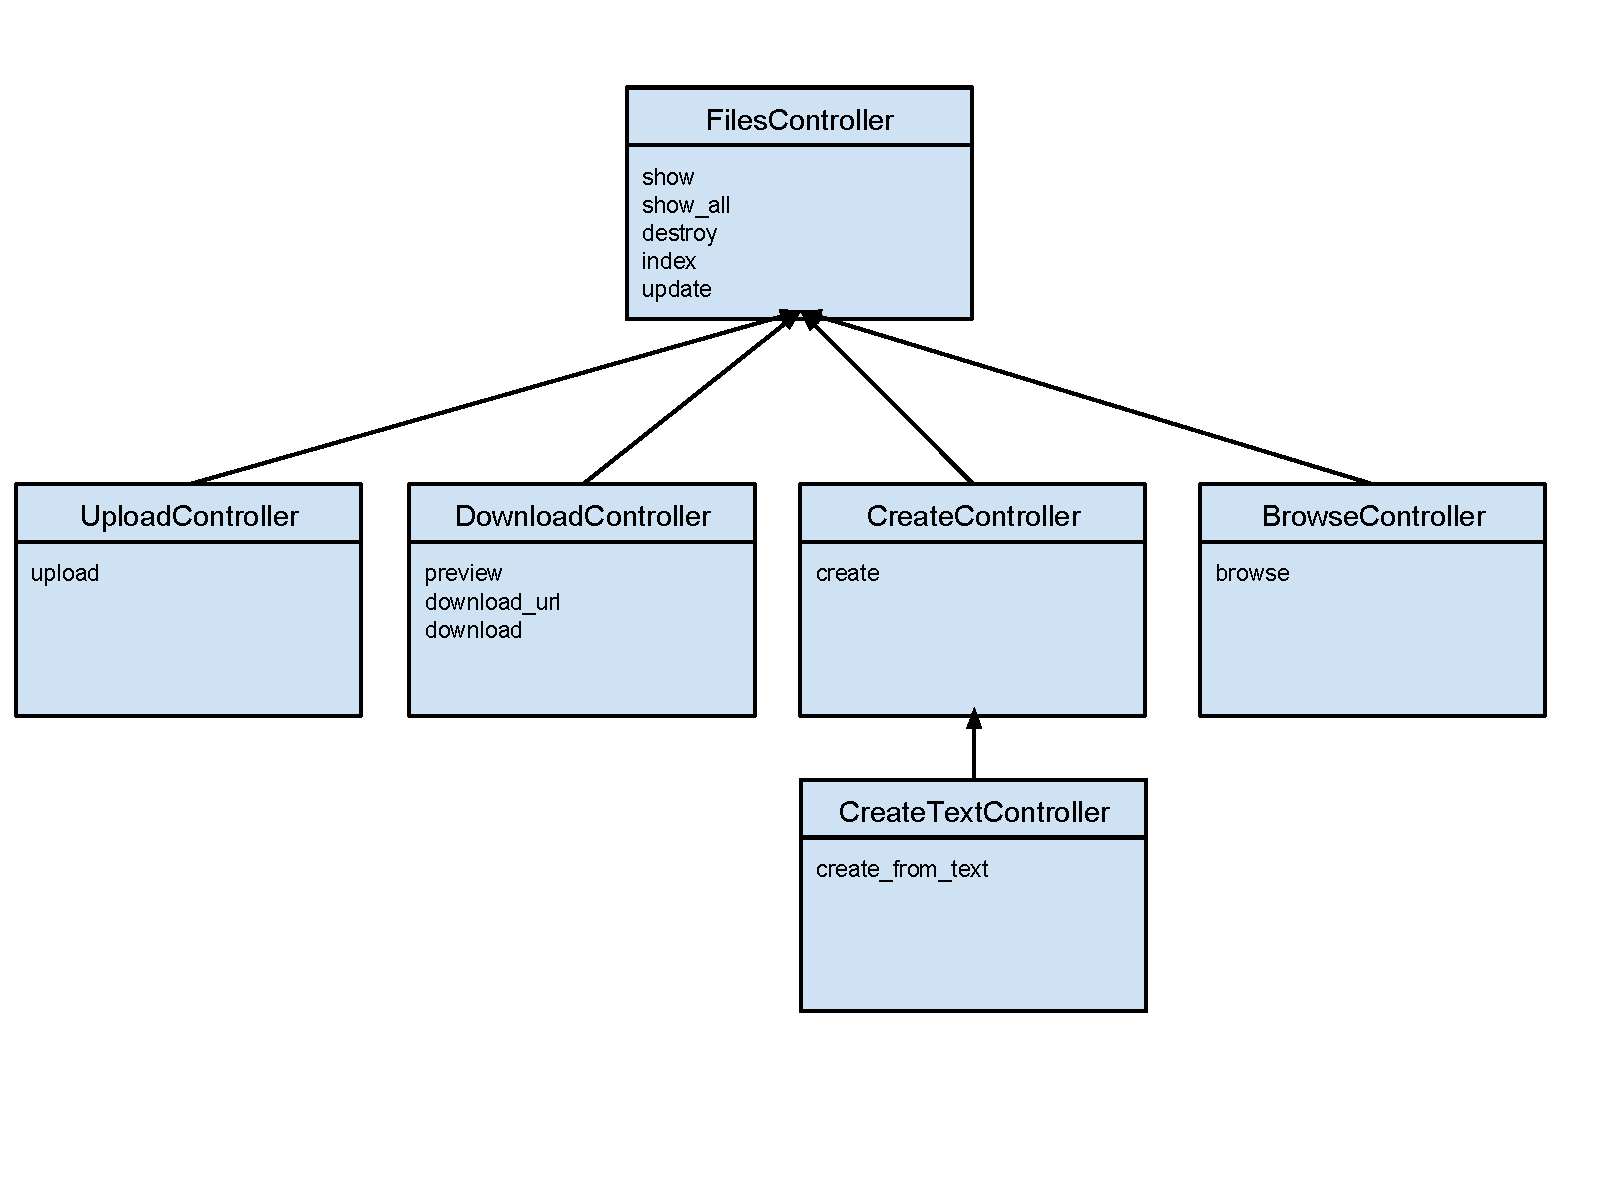
\includegraphics[width=0.9\linewidth]{figures/filescontroller.pdf}
    % caption! change the label ref to what you want
    \captionof{figure}{\emph{Struktur för filrelaterade \emph{controllers}.}\label{fig:filescontroller}}
\end{Figure}

\subsubsection{\texttt{FilesController}}

Denna \emph{controller} är den som alla ärver av, som kan ses i figur
\ref{fig:filescontroller}. Den hanterar de vanligaste metoderna för en fil, de
som handlar om att hitta eller redigera den information om filer som redan är
sparad i databasen. Skillnaden mellan funktionerna \emph{index} och \emph{
show\_all} är att \emph{index} visar alla filer för en identity vid import
medans \emph{show\_all} visar alla filer för alla användarens identities.

\subsubsection{\texttt{BrowseController}}

Hanterar inläsning av mappar från en extern tjänst.

\subsubsection{\texttt{CreateController}}

Skapar ett nytt inlägg i databasen från den information som fås av klienten.
Här finns även validering så att endast tillåtna variabler skickas vidare till
att sparas i databasen. Valideringen av vilken typ variablerna är sker senare i
systemets \emph{model} \texttt{BruseFile}.

\subsubsection{\texttt{CreateTextController}}

Ärver av \texttt{CreateController}. Denna \emph{controller} skapades då
\texttt{create\_text} kräver många fler hjälpfunktioner och valet gjordes att
dela upp dem för att hålla det strukturerat. Många av de funktionerna handlar
om att hantera textsträngen om den är en URL.

\subsubsection{\texttt{DownloadController}}

För att ladda ner filer på ett säkert sätt som kräver att rätt användare är
inloggad skapades en \emph{controller} för att säkerställa detta med ett antal
funktioner. Funktionen \texttt{preview} fick även vara i denna då den hanterar
filer på ett liknande sätt som \texttt{download} gör. \texttt{download\_url}
skapades för att eventuellt implementera en delningsfunktion där flera
användare skulle kunna få tillgång till filen.

\subsubsection{\texttt{UploadController}}

Hanterar filer som ska laddas upp till de olika tjänsterna. Om filen laddas upp
via drag och släpp-metoden eller via ett vanligt formulär tas filerna emot i
olika format. Via drag och släpp-metoden fås filen kodad i \emph{base64}
vilket måste göras om till en så kallad \texttt{Tempfile} och sedan till ett
objekt som är samma som det som fås via formulärsuppladdning \cite{base64}.

\subsection{Klient – Angularjs}

Tillsammans bildar filerna olika komponenter som används för att hantera sina områden, se figur \ref{fig:angularstructure}. De områden som styrs utav Angularjs är

\begin{itemize}
  \item lägga till filer
  \item lägga till taggar till nyligen tillagda filer
  \item söka efter filer
  \item skapa filer från text
  \item drag och släpp-uppladdning
  \item lista filer.
\end{itemize}

\begin{Figure}
  % center it!
  \centering
    % adjust width as you like, include image from optional folder
    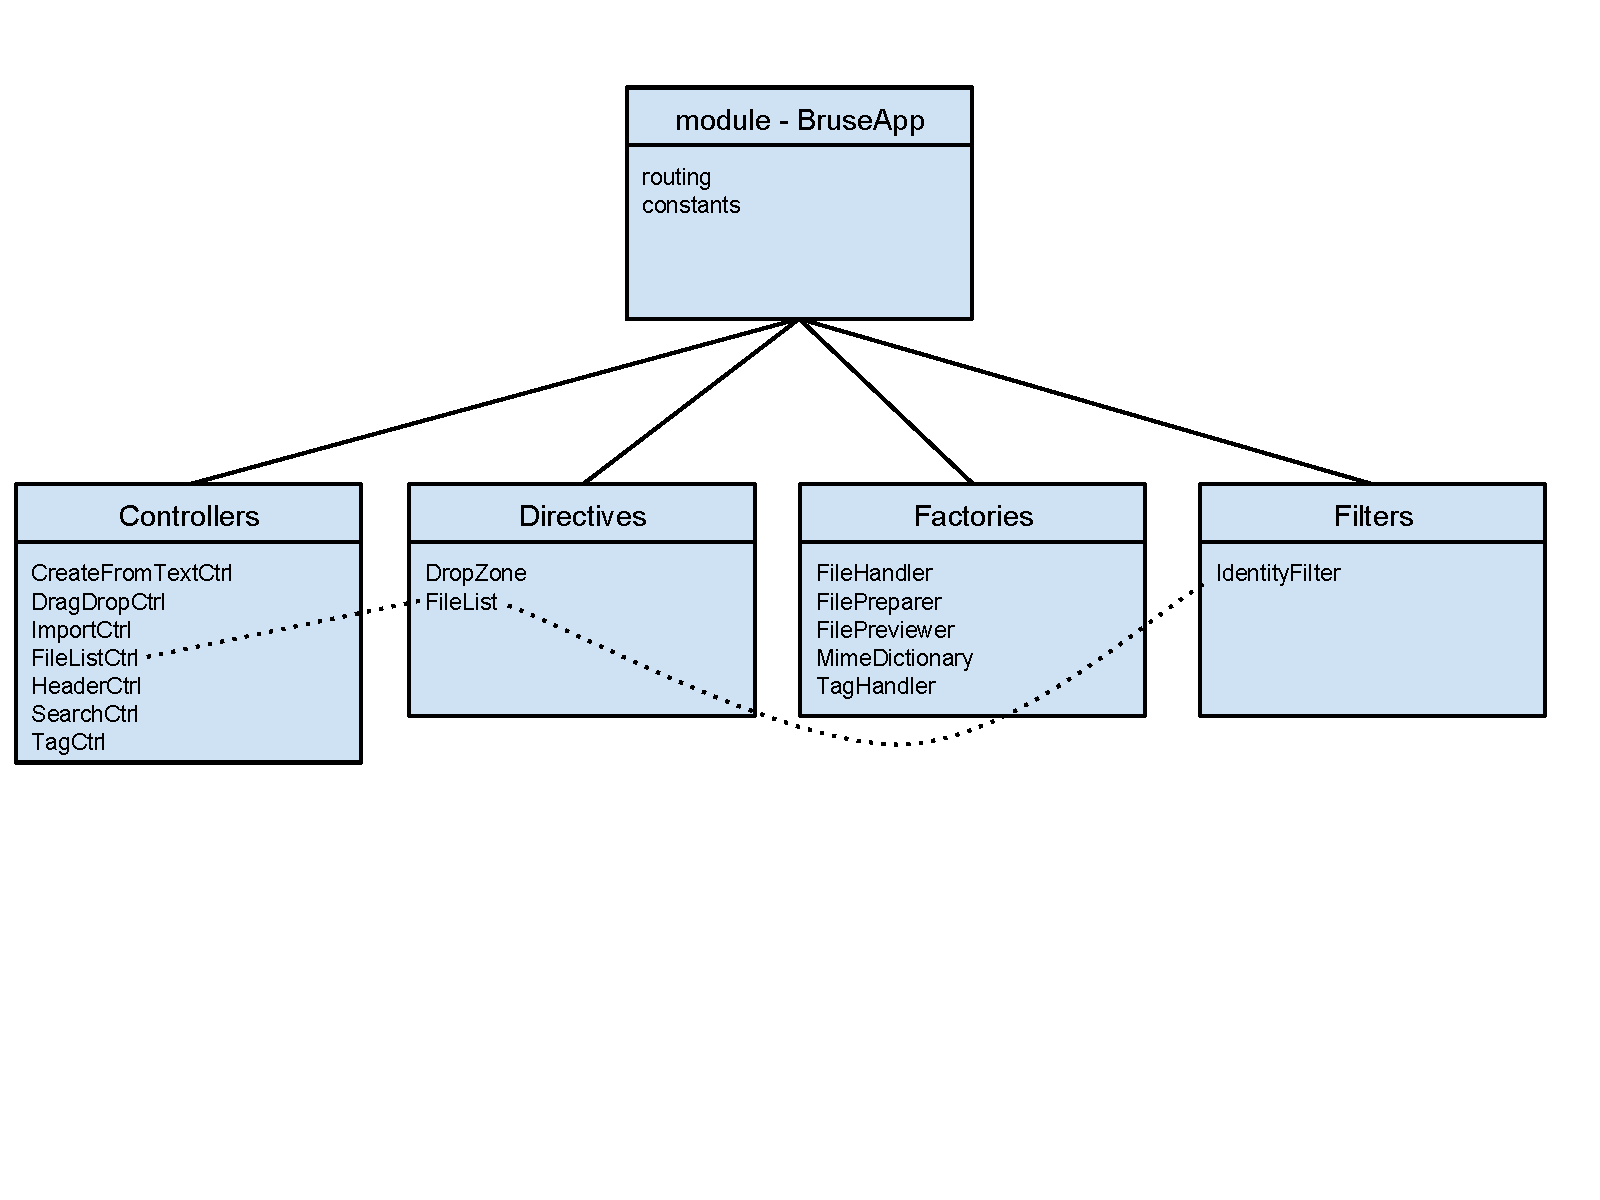
\includegraphics[width=0.9\linewidth]{figures/angularstructure.pdf}
    % caption! change the label ref to what you want
    \captionof{figure}{\emph{Struktur för Angularjs-komponenter.}\label{fig:angularstructure}}
\end{Figure}

Vid import av filer sparas alla de valda filerna i en \emph{array} i
Javascript, sedan när användaren väljer att spara filerna skickas en förfrågan
till serven per fil för att lägga till dem i databasen. Denna \emph{array}
sparas i en global variabel som Angularjs tillhandahåller. Användaren
omdirigeras genom att systemet byter HTML-\emph{template} och URL för att ge
intrycket av att användaren kommer till en ny sida. Men då det är samma session
och ingen ny förfrågan mot serven har gjorts av webbläsaren kan denna nya sida
komma åt samma globala variabel och på så sätt använda sig av de nyligen
tillagda filerna.

Denna lösning använder sig av ett verktyg för Angularjs som heter Angular
Router. Detta verktyg kan hantera olika URL-förfrågor i Javascript och
presentera \emph{templates} och \emph{controllers} som utvecklare specificerat.
Men då en förfrågan av en webbläsare sker först till serven måste även Angular
Router-systemet där vidarebefodra vissa förfrågor till en speciell URL så att
Javascript och Angular Router kan ta över istället för servern.

Angularjs \emph{factories} användes för att: uppdatera och skapa filer, för att visa
filer, för att uppdatera taggar, för att förbereda filer för visning samt för
att hantera olika filtyper. Detta kan exempelvis innebära att
\texttt{MimeDictionary.prettyType()} användes för att skriva ut en fils MIME-
typ (\emph{Multipurpose Internet Mail Extensions}) i ett mer läsbart format
\cite{mime}. Exempelvis ``excel spreadsheet'' istället för
``application/vnd.ms-excel'' och ``c++ file'' istället för ``text/x-c''.

\emph{Factories} användes även för att hantera asynkrona anrop mot servern.
Detta gjorde att utvecklaren kunde veta när anropen var färdiga, till exempel
när en fil hade uppdaterats och vad resultatet blev.

\subsection{Sökning}

\begin{Figure}
  % center it!
  \centering
    % adjust width as you like, include image from optional folder
    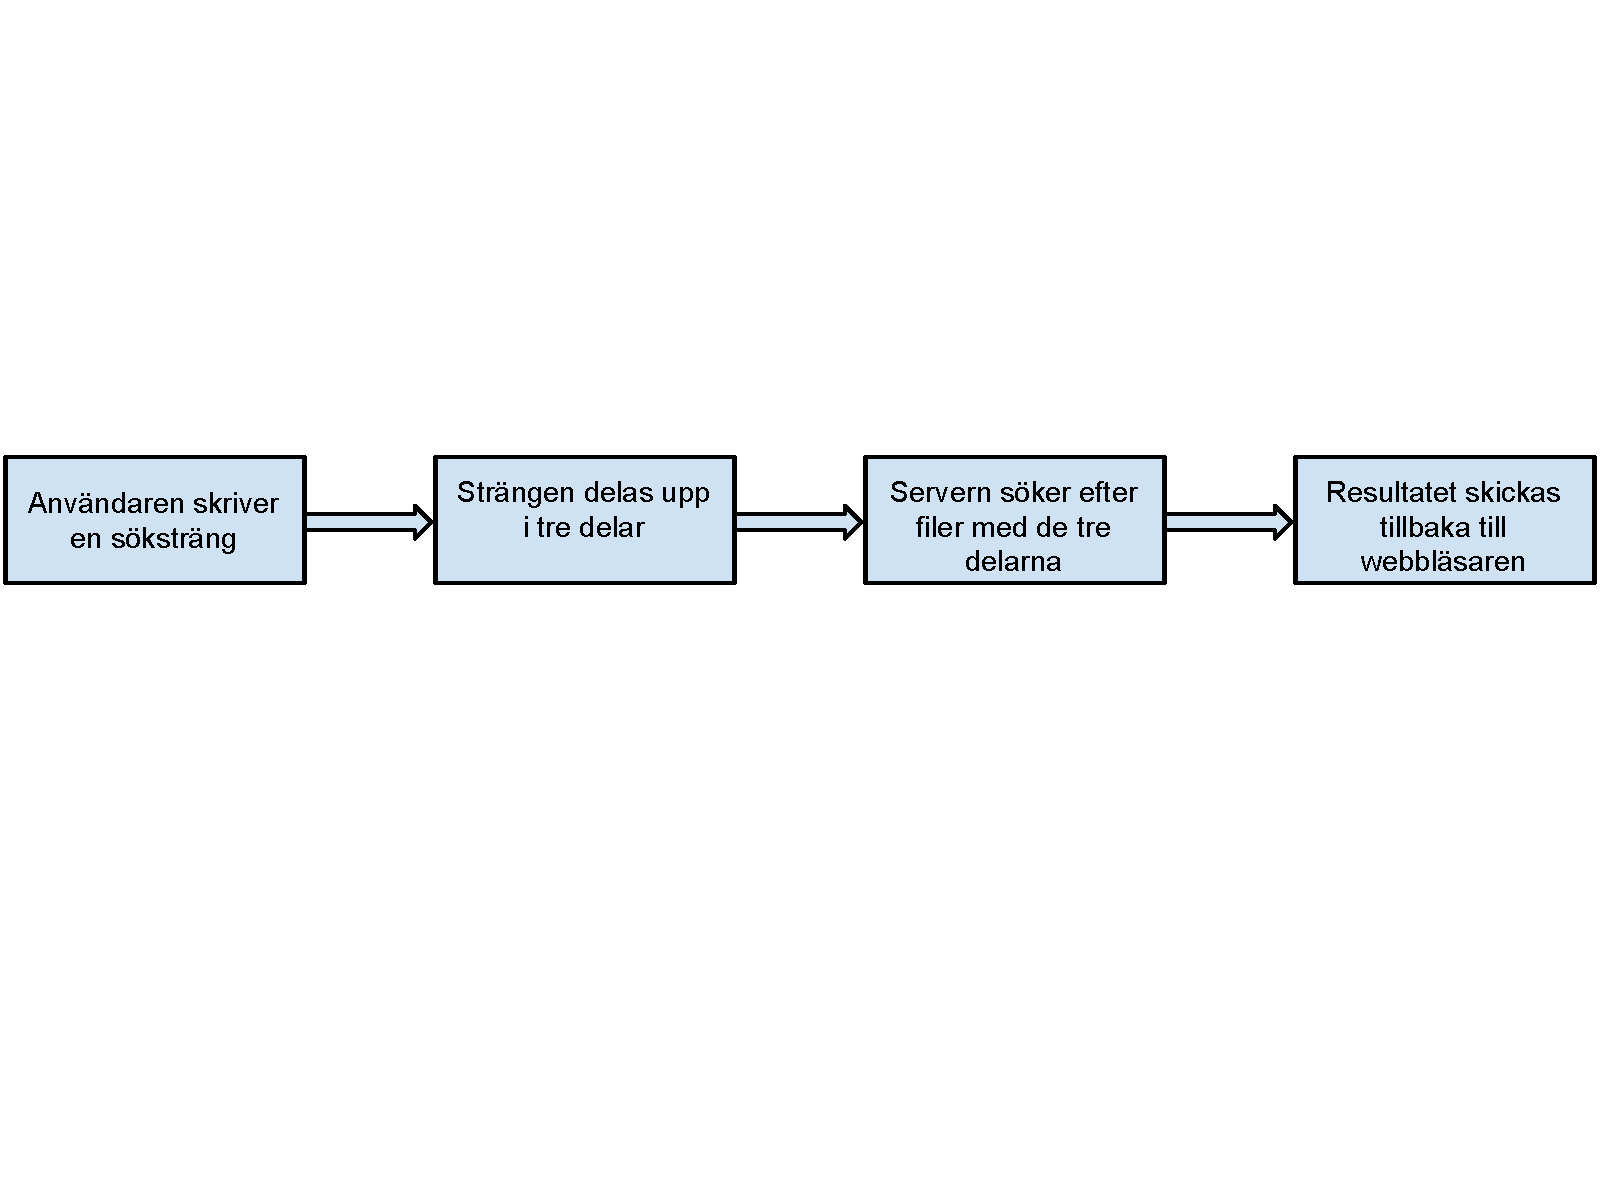
\includegraphics[width=0.9\linewidth]{figures/search.pdf}
    % caption! change the label ref to what you want
    \captionof{figure}{\emph{Flöde över sökning.}\label{fig:search}}
\end{Figure}

För att låta en användare söka efter filer i systemet på ett enkelt och
effektivt sätt delades denna funktion upp så att både servern och klienten
användes för att hantera användarens önskemål. Hos klienten skrev användaren in
sin söksträng som en kombination av ord, ord föregångna av ett nummertecken
``\#'' och ord föregågna av en punkt ``.''. Denna söksträng delades upp efter
respektive typ av ord, och skickades till servern. Servern tog då hand om denna
samling som generella ord att söka efter, taggar att söka efter samt filtyper
att söka efter. Då en användare skrev söktermen ``hej \#hälsning .txt'' sökte
alltså servern efter filer och taggar som innehöll ordet ``hej'' i sitt namn,
hade taggen hälsning och var en textfil. Resultatet presenterades sedan för
användaren utav klienten. Figur \ref{fig:search} visar en översikt över
sökningen.

\section{Tredjepartsmjukvara}

Devise är ett tillägg till Ruby on Rails som ger ett paket för
användarhantering, färdigt att användas. Då beslutet om att användare även
skulle kunna logga in med e-postadress och lösenord insågs det samtidigt att en
tredjepartsmjukvara skulle vara nödvändigt för att hålla tidsramen. Devise
valdes för att det gav den mest kompletta lösningen med färdiga \emph{views},
modifierbara \emph{controllers} och enkel \emph{model}-påbyggnad. Devise har
också inbyggda funktioner som tillsammans med Rails e-postssystem skickar e-
post till användare då de till exempel registrerar sig eller behöver hjälp med
att återställa sitt lösenord.

Carrierwave ger utvecklarna verktyg för att hantera uppladdningen av filer.
Genom att endast specificera inställningar för var filen ska sparas och så
vidare fås en modul som kan användas i de \emph{controller}-metoder som behövs.

Fuzzily skapar för varje ny instans av specificerade models så kallade
\emph{trigrams} över valda kolumner. \emph{Trigrams} delar upp ett ord och
grupperar det om tre tecken i taget \cite{n-grams}. För varje ny gruppering
förflyttas den ett steg vilket gör att det skapas flera olika kombinationer.
För ett ord skulle det resultera i flera olika bokstavskombinationer av
grundordet. Exempelvis skulle ordet ``bruse'' med hjälp av trigrams bli
\texttt{[b, br, bru, rus, use, se, e]}. Under implementationen av Fuzzily
upptäcktes det att  numeriska eller nordiska tecken inte sparades i trigrams.
Tack vare att Fuzzily är skrivet i öppen källkod kunde problemet åtgärdas genom
att ändra koden.

Delayed Job användes för att kunna skjuta upp skapandet av \emph{trigrams}.
Genom att spara kommande jobb i en lista kunde skapandet ske utan att blockera
en förfrågan från användaren. Istället skedde detta i en ny process i
bakgrunden.

Jstag är ett tillägg till Angularjs som konverterar användarens inskrivning
utav taggar till visuella objekt för att tydliggöra för användaren hur dess
inskrivning tolkas utav systemet. Även detta tillägg hade brister då olika
objekt kopierades utav systemet utan att samtliga tvåvägsbindningar behölls som
kunde åtgärdas tack vare att det var skrivet med öppen källkod.

Magnific Popup gör att filerna som laddas upp till systemet går att
förhandsgranska i samma vy som användaren befinner sig på. För att en viss
filtyp ska kunna förhandsgranskas krävs det att man lägger till en definition
för filtypen i hjälpfunktionen \texttt{MimeDictonary}. Magnific Popup använder
samma teknik som webbläsaren gör för att förhandsgranska en fil vilket gör att
filtyper som bilder, filmer, musik och textfiler går att öppna.

\subsection{Filhantering}

Då en fil lagrades i systemet var det två attribut som var centrala. Dels
varifrån filen sparats – om den importerades från en extern tjänst som Google
Drive eller Dropbox, eller om den lagrades i systemets lokala fillagring. Dels
också en textsträng som motsvarar hur den aktuella tjänsten som filen tillhör
separerar filen från övriga filer . Denna textsträng kallas i systemet för
\texttt{foreign\_ref}. För Google Drive är detta en slumpmässig bokstavs- och
sifferkombination, för Dropbox är detta sökvägen till filen. För den lokala
filhanteringen är detta namnet på filen efter att den sparats på servern, också
detta en slumpad bokstavs- och sifferkombination.

\subsection{Gränssnitt}

Systemet utvecklades för att ge användaren en enkel och tillgänglig upplevelse
med ljusa färger och tydliga uppdelningar mellan systemets komponenter. Nedan
visas skärmdumpar från systemets olika delar. I figur \ref{fig:dump1} till
\ref{fig:dump5} visas skärmdumpar från systemet.

\begin{Figure}
  % center it!
  \centering
    % adjust width as you like, include image from optional folder
    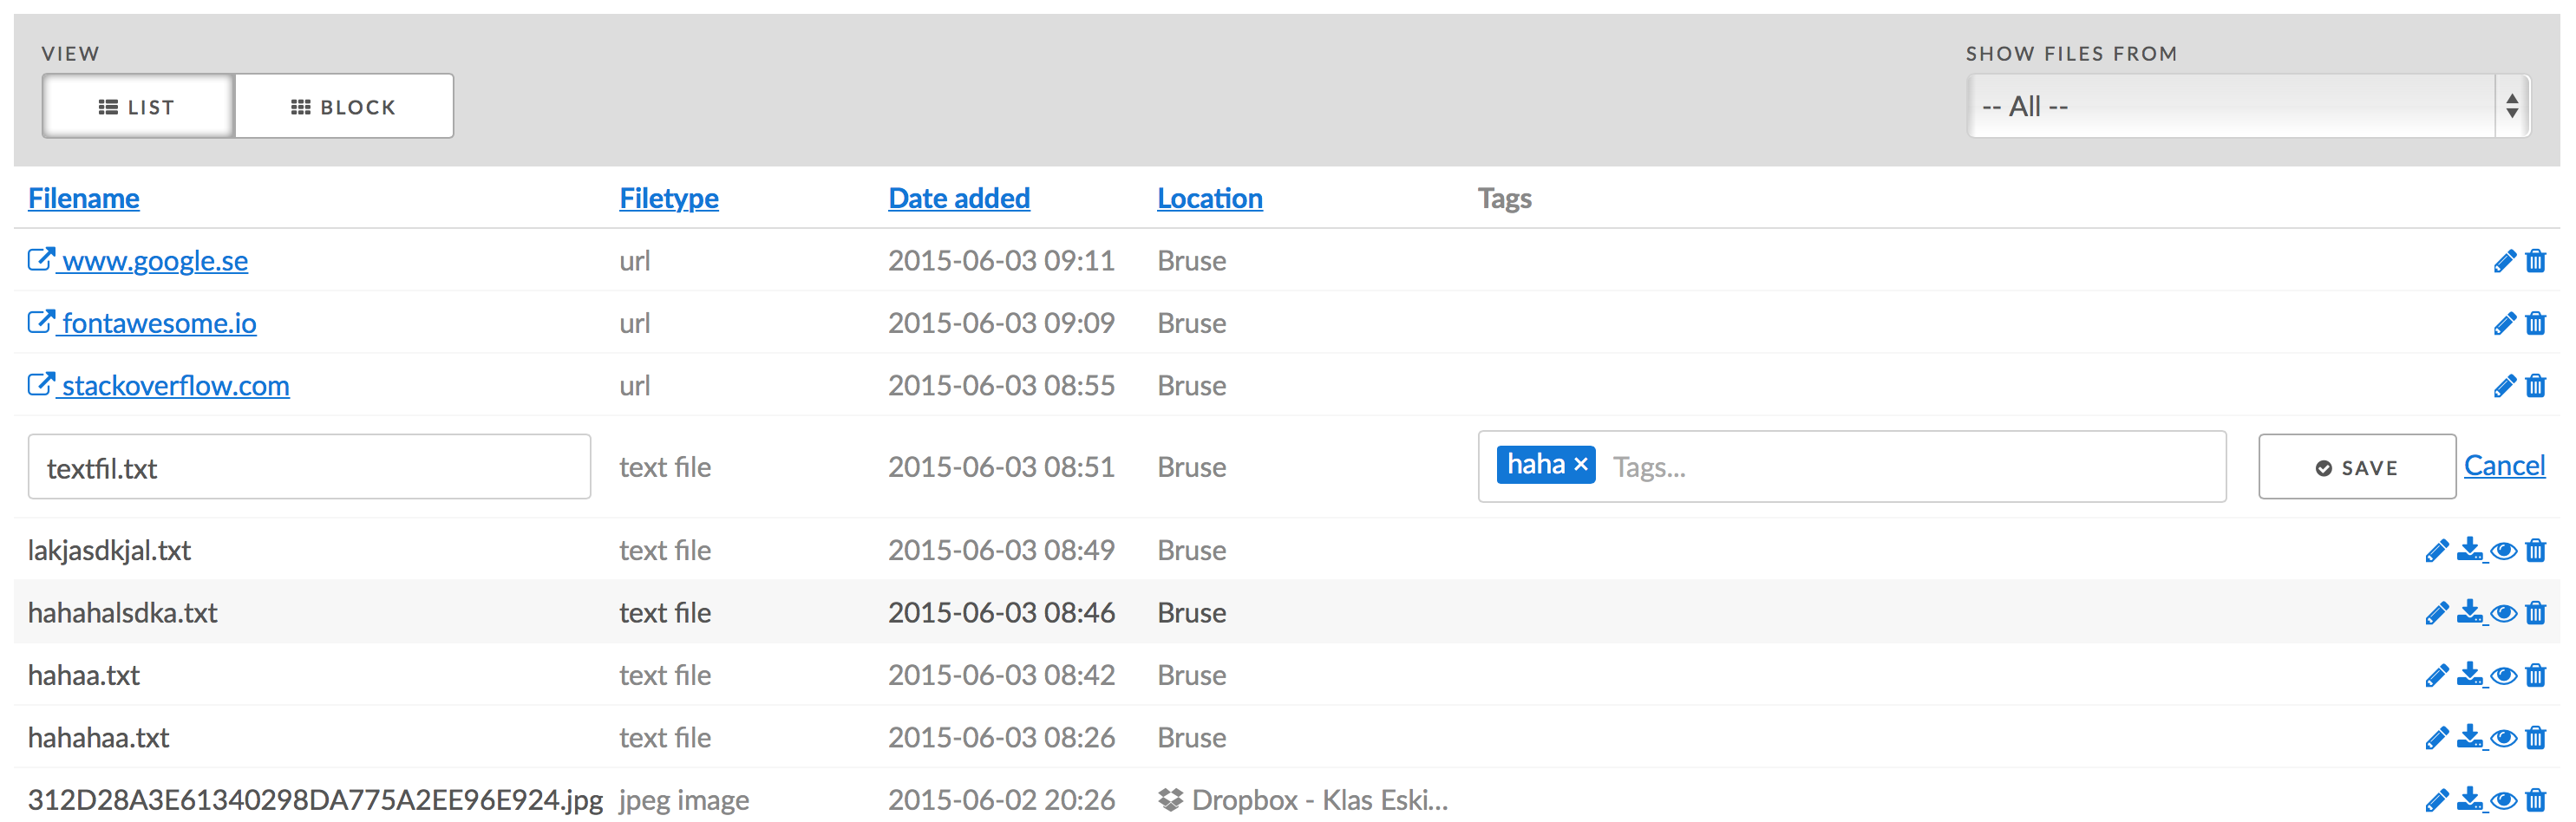
\includegraphics[width=0.9\linewidth]{figures/screenshots/dump1.png}
    % caption! change the label ref to what you want
    \captionof{figure}{\emph{Systemets lista över dess filer. En fil redigeras.}\label{fig:dump1}}
\end{Figure}

\begin{Figure}
  % center it!
  \centering
    % adjust width as you like, include image from optional folder
    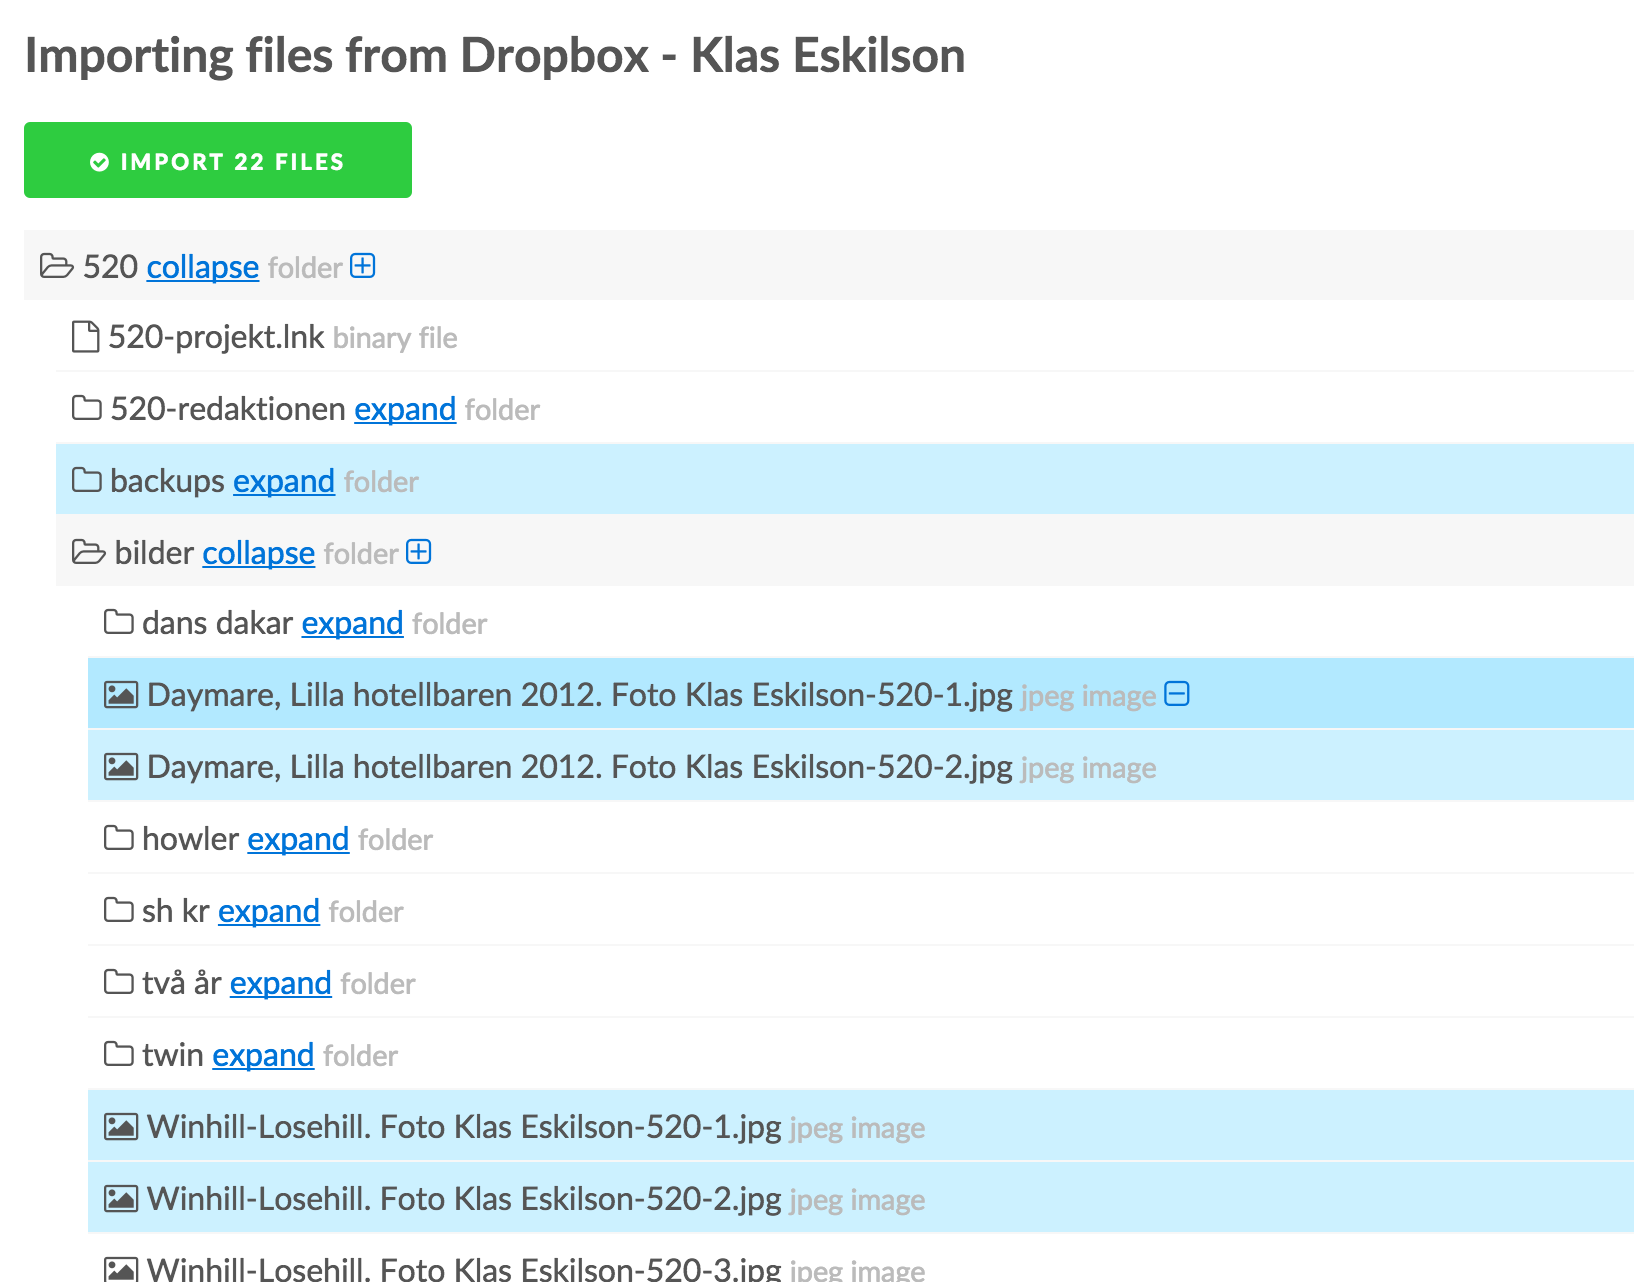
\includegraphics[width=0.8\linewidth]{figures/screenshots/dump2.png}
    % caption! change the label ref to what you want
    \captionof{figure}{\emph{Filimport.}\label{fig:dump2}}
\end{Figure}

\begin{Figure}
  % center it!
  \centering
    % adjust width as you like, include image from optional folder
    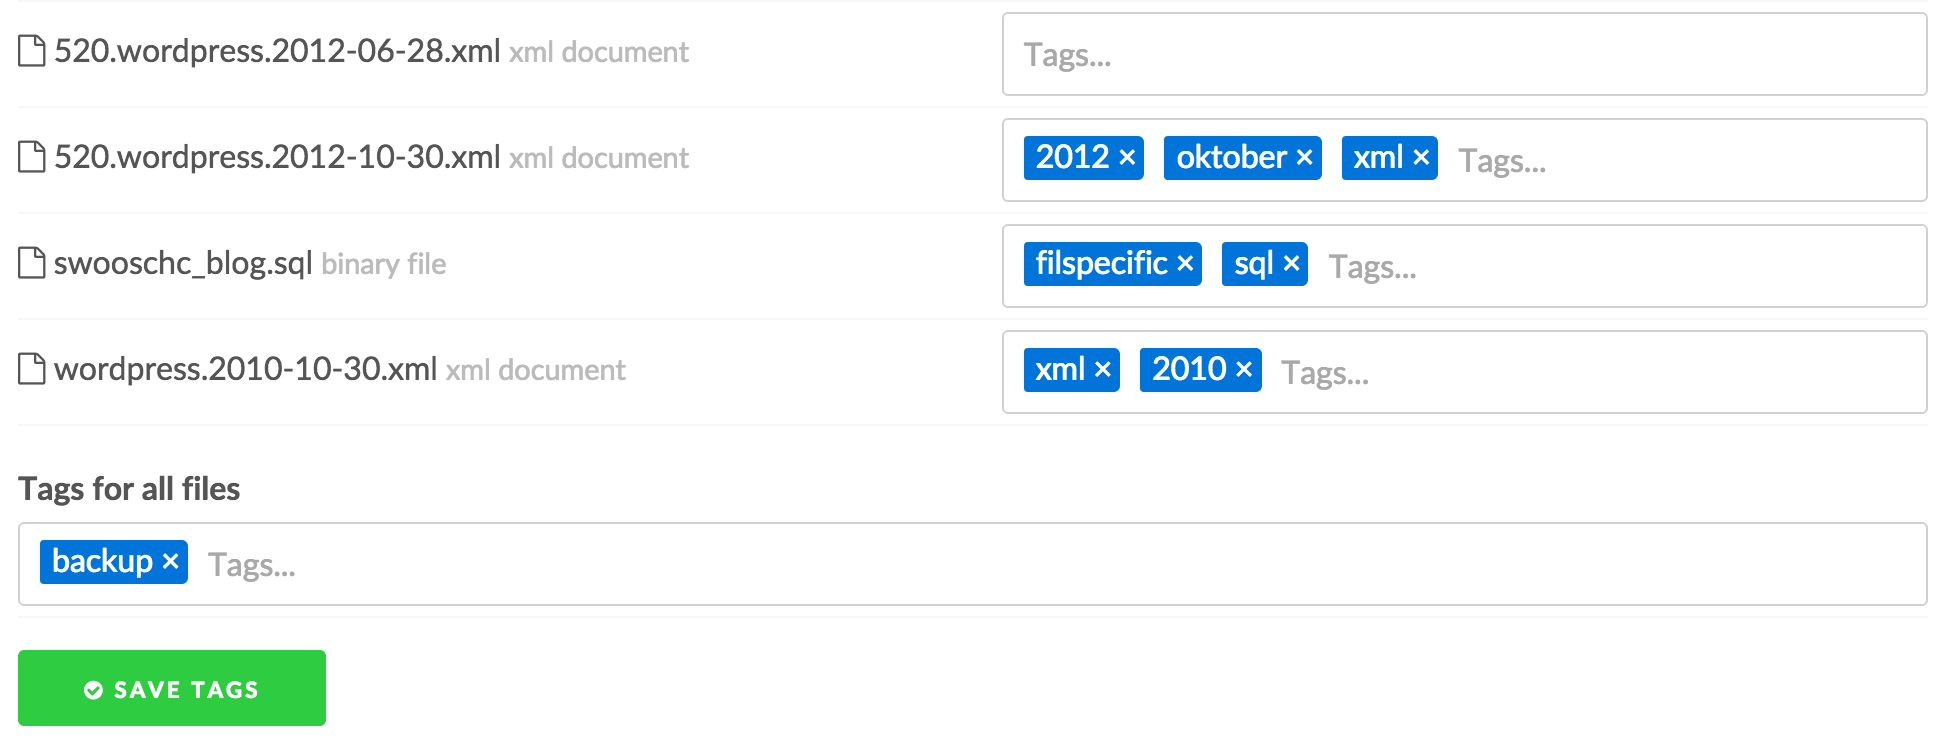
\includegraphics[width=0.7\linewidth]{figures/screenshots/dump3.png}
    % caption! change the label ref to what you want
    \captionof{figure}{\emph{Taggning av filer efter import.}\label{fig:dump3}}
\end{Figure}

\begin{Figure}
  % center it!
  \centering
    % adjust width as you like, include image from optional folder
    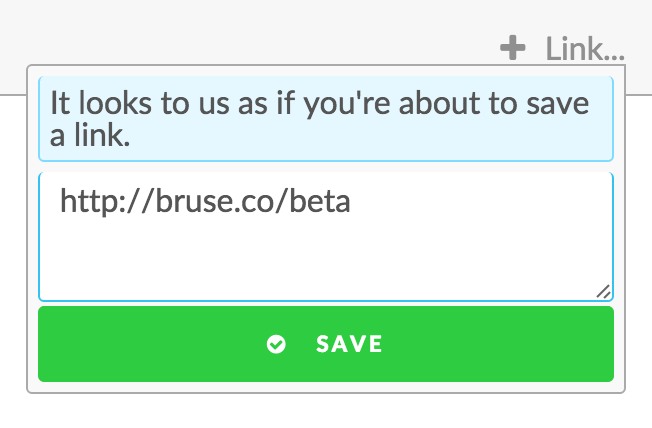
\includegraphics[width=0.4\linewidth]{figures/screenshots/dump4.png}
    % caption! change the label ref to what you want
    \captionof{figure}{\emph{Sparande av bokmärke via textfält.}\label{fig:dump4}}
\end{Figure}

\begin{Figure}
  % center it!
  \centering
    % adjust width as you like, include image from optional folder
    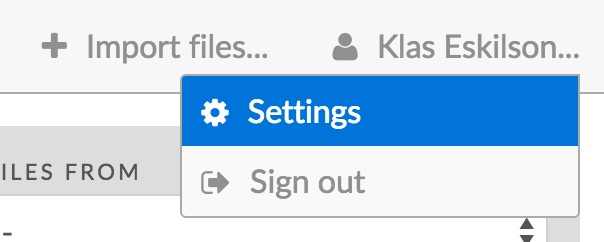
\includegraphics[width=0.4\linewidth]{figures/screenshots/dump5.png}
    % caption! change the label ref to what you want
    \captionof{figure}{\emph{Öppen undermeny.}\label{fig:dump5}}
\end{Figure}

\section{Utvecklingsmetodik}

Arbetet följde Scrum som utvecklingsmetodik vilket har resulterat i en tydlig
och strukturerad arbetsgång. Korta scrummöten i början av varje arbetsdag har
förhindrat onödigt arbete samt att alla utvecklare är insatta i arbetet. Varje
sprintgranskning och sprintåterblick har givit en tydlig bild om vad som gjorts
och behöver göras för att nå nästa förbättring av produkten.

\section{Versionshantering och kodgranskning}

Användningen av Github gjorde att det alltid fanns en fungerande programversion
i \emph{develop}-förgreningen. Systemet växte i funktionalitet allt eftersom
nya tillägg från \emph{pull requests} godkändes. Om det inte fanns behov av
kodning fanns det alltid behov av att granska \emph{pull requests}. Antal
\emph{pull requests} och \emph{commits} varierade från person till person.
\emph{Commits} från varje gruppmedlem och övrig statistik finns i bilaga [].


\chapter{Analys och diskussion}

\section{Metod}

\subsection{Systemarkitektur}

\subsection{Filhantering}

\subsection{Hantering och strukturering av databaser}

\subsection{Gränssnitt}

\subsection{Testning}

\subsection{utvecklingsmetodik}

\subsection{Versionshantering och kodgranskning}

\section{Resultat}

\subsection{Filhantering}

\subsection{Tredjepartsverktyg}

\section{Arbetet i ett vidare sammanhang}

\subsection{Fildelning}

\subsubsection{Filhantering}

\subsubsection{Olagliga filer}

\subsubsection{Personlig integritet}

\chapter{Slutsatser}

\section{Frågeställningar}

\subsection{Struktur på webbdatabas}

\textbf{Hur ska en webbdatabas struktureras för att sökning efter sparade objekt
ska kunna levereras enligt en användares förväntningar om hastighet och
resultat?}

Genom att dela upp taggar för sig och filer för sig och skapa en relation mellan
de två som förklaras i sektion. Användaren kan specificera om den vill söka på
taggar, filer eller båda två. Om det specificeras vilken typ som söks efter
kommer systemet att kunna leverera ett snabbare resultat.

\subsection{Säkerhet}

\textbf{Hur går det att säkerställa att en användares information som lagras i
en webbdatabas inte är tillgänglig för någon som inte är den specifika
användaren eller har blivit  auktoriserad av den specifika användaren?}

Genom att arbeta med en säker sessionshantering på servern som gör att en
användare inte kan mixtra med en serverförfrågan för att ändra inlogg. För att
ingen ska kunna få ut någon annan användares information måste systemet
försäkras om att rätt användare är inloggad och inte vara beroende på vilket id
som skickas med i en serverförfrågan. På så sätt kan endast de inlägg i
databasen som är kopplade till rätt användar-id säkert presenteras och .

\subsection{Databasbaserad filstruktur}

\textbf{Hur kan filer i en webbdatabas presenteras i en webbapplikation på ett
sätt som gör de överskådliga,  hanterbara och lättillgängliga för en användare,
i en filstruktur utan kataloger eller annan hierarki?}

Filer i en webbdatabas kan presenteras genom en databasbaserad filstruktur i en
webbapplikation. En databasbaserad filstruktur innebär att filerna visas
vartefter de söks efter med hjälp av taggar eller metadata. På så sätt kan
filerna lätt hittas, så länge användaren vet på ett ungefär vad den letar efter.
Filer som stämmer överens med alla sökord genom en \emph{fuzzy search} visas.
Användaren kan också redigera filens taggar till att passa sökningen bättre.

\subsection{Användargränssnitt}

\textbf{På vilket sätt kan en webbapplikations användargränssnitt designas för
att demonstrera all funktionalitet ett system besitter och göra det intuitivt
för en användare?}

\section{Framtida arbete}

I nästa version av rapporten, efter att den sista sprinten är klar, kommer
användargränssnittet beskrivas då det inte är färdigt ännu.

Den framtida visionen för systemet är att fler användare ska kunna interagera
med varandra genom att dela filer, projekt eller mood boards med varandra.
Systemet ska möjligtvis kunna användas genom ett Chrome plugin som gör det
snabbare att söka efter filer.

För att öka säkerheten och kunna lagra filer på ett effektivare sätt kan den
framtida databashanteringen ske med hjälp av MongoDB.

Box!

\subsection{Slutgiltigt rapportförslag}
Denna rapport tar inte upp någonting om systemets användargränssnitt. Det beror
på att gränssnittet i skrivande stund ej var färdigutvecklat.



\begin{thebibliography}{99}
\addcontentsline{toc}{chapter}{\bibname}

\bibitem{gettingthingsdone}
  D. Allen, \emph{Getting Things Done: The Art of Stress-Free Productivity}, Penguin Books 2001

\bibitem{softwareeng}
  Shari Lawrence Pfleeger och Joanne M. Atlee, \emph{Software Engineering, Fourth Edition, International Edition}, Pearson 2010

\bibitem{tagging}
  J. Granström, \emph{Social taggning}, Högskolan i Borås 2007, hämtad: 2015-04-08\newline http://bada.hb.se/bitstream/2320/2178/1/07-56.pdf

\bibitem{norman}
  C. Kroner Grogarn, K. Olin, M. Sun Bursjö, \emph{Hur långt når Norman?}, Göteborgs universitet 2011, hämtad: 2015-05-14\newline https://gupea.ub.gu.se/bitstream/2077/26683/1/gupea\_2077\_26683\_1.pdf

\bibitem{whitespace}
  K. Lahtinen, \emph{Skapandet av en modern webbdesign}, Arcada 2014, hämtad: 2015-05-14\newline http://www.theseus.fi/handle/10024/73920

\bibitem{twente}
  O. Gorter, \emph{Database File System: An Alternative to Hierarchy Based File Systems}, University of Twente 2004, hämtad: 2015-05-14\newline https://www.sphinux.org/misc/docs/references/papers/dbfs.pdf (hämtad 2015-04-27)

\bibitem{rubylang}
  D. Flanagan, Y. Matsumoto, \emph{The ruby programming language}, O'Reilly Media, Inc. 2008

\bibitem{angularjs}
  R. Branas, \emph{AngularJS Essentials}, Packt Publishing Ltd. 2014

\bibitem{sqlenc}
  Encyclopædia Britannica. Encyclopædia Britannica Online. Encyclopædia Britannica Inc., 2015. Web. 12 maj. 2015 <http://global.britannica.com/EBchecked/topic/569684/SQL>.

\bibitem{objrel}
  Płuciennik-Psota, E. \emph{Object relational interfaces survey}. Studia Informatica, 2012.

\bibitem{proar}
  Pytel, C., Yurek, J., och Marshall, K.. \emph{Pro Active Record: Databases with Ruby and Rails}. Apress, 2007.

\bibitem{indexes}
  Aoki, P. M. \emph{Implementation of extended indexes in POSTGRES.} SIGIR Forum, vol. 25, no. 1, ACM, 1991.

\bibitem{rubychangelog}
  Minitest in Ruby, hämtad 2015-05-14.
  \newline<http://svn.ruby-lang.org/repos/ruby/tags/v1\_9\_1\_0/NEWS>.

\bibitem{scrumguide}
  K. Schwaber, J. Sutherland, \emph{Scrumguiden}, 2013-07, hämtad: 2015-05-13\newline http://www.scrumguides.org

\bibitem{progit}
  S. Chacon och B. Straub, \emph{Pro Git}, 2nd ed., 2014

\bibitem{gitflow}
  Preißel, R., Stachmann, B., \emph{Git: Distributed Version Control--Fundamentals and Workflows}, dpunkt.verlag, 2014.

\bibitem{}
\bibitem{}
\bibitem{}
\bibitem{}
\bibitem{}
\bibitem{}
\bibitem{}
\bibitem{}
\bibitem{}
\bibitem{}

\end{thebibliography}


\appendix

\chapter{Bilaga}


\end{document}
